\documentclass[12pt, ChapStyle1, oneside]{./Styles/Dea_Gsm}
\usepackage{graphicx}
\usepackage{color}
\usepackage[T1]{fontenc}
\usepackage{amsfonts}
\usepackage{textcomp}
\usepackage{setspace}
\usepackage{hyperref}
\usepackage{float}
\usepackage{array}
\usepackage{tabu}
\usepackage {longtable}
\usepackage{mathrsfs, amsmath, amssymb, bbm}
\usepackage{pstricks, pst-node, pst-tree, pstcol}
\usepackage[dvips]{epsfig}
\usepackage{floatflt,multirow, subfigure, hhline, enumerate, comment, url, pifont}
\usepackage[active]{./Styles/srcltx,rotating}
\usepackage[ruled,vlined,french,titlenumbered]{algorithm2e}
\usepackage{listings}


\graphicspath{{./images/}}
\hyphenpenalty=10000
\hypersetup{
    colorlinks,
    citecolor=black,
    filecolor=black,
    linkcolor=black,
    urlcolor=black
}

\pagenumbering{arabic}
\usepackage[normalem]{ulem}
\setcounter{section}{1}
\setcounter{secnumdepth}{5}

\begin{document}

\Remerciements{DÉDICACE}
\vspace{8mm}
\Large
\begin{center}
\texttt{
Ce travail est dédié :
\vspace{6mm}
\\*À mes très chers parents qui ont toujours
été là, à mes côtés, tout au long de mes études et qui ont été pour moi,le modèle idéal de courage et persévérance, et qui j'espère, trouveront dans ce travail toutes ma reconnaissance et tout mon amour,
\\*À mes sœurs, pour l'amour et la tendresse qu'elles n'ont cessé de m'apporter, réunies comme lors de notre éloignement, pendant toute la durée de ma formation et à mes amis qui m'ont apporté leur soutien.
\\*À vous tous je dis:
\\*Je vous aime du plus profond de mon coeur.}
\end{center}
\vspace{6mm}
\begin{flushright}
\Large Marwen
\end{flushright}

\Remerciements{REMERCIEMENTS}
\large
C'est avec plaisir que je réserve ces quelques lignes en signe de gratitude et de profonde reconnaissance à tous ceux qui, de près ou de loin, ont contribué à l'aboutissement de ce travail.

\vspace{4mm}
Je tiens à exprimer mes vifs remerciements en premier lieu à Monsieur\textbf{ Skander DOUKI}, Directeur de \textbf{Pixels Trade} pour m'avoir accueilli au sein de son unité.

\vspace{4mm}
Je tiens à remercier mon superviseur Monsieur \textbf{Mohamed Ali RAHALI} pour son aide, ces conseils précieux, ces critiques constructives et ces suggestions pertinentes qui ont été remarquables tout au long de mon stage.

\vspace{4mm}
J'adresse aussi mes profonds remerciements à Monsieur \textbf{Sadok BEN YAHIA}, mon encadreur au sien de la Faculté des Sciences de Tunis, pour son encadrement, son soutien, sa disponibilité et ses conseils qui m'ont guidé tout au long de mon stage.

\vspace{4mm}
Je remercie également tous les membres de l'équipe de Pixels Trade, pour leur collaboration très fructueuse que j'ai eu pendant l'avancement de mon travaux.

\vspace{4mm}
Enfin, Je suis reconnaissant à tout le personnel et le corps professoral de la Faculté des Sciences de Tunis et à tous ceux, qui m'ont apporté de l'aide même minime. Je saisis cette occasion pour remercier les membres du jury tout en espérant qu'ils trouvent dans ce rapport les qualités de clarté et de motivation qu'ils attendent.
\tableofcontents
\pagebreak
\listoffigures
\pagebreak
\Introduction{Introduction générale}
\setcounter{page}{1}
\vspace{5mm}
\PARstart{L}{'essor} des nouvelles technologies ainsi que les progrès effectués dans le domaine des télécommunications, des réseaux et du traitement de l’information, ont engendré l’apparition de nouveaux outils et objets communicants comme les smart phones, les tablettes, les IPads, etc. 
Notre environnement quotidien a connu une mutation en devenant un environnent intelligent, qui assure le raffinement des services de communications avec les équipements audiovisuels. En outre, ces équipements proposent des applications qui peuvent servir tous les domaines de travail. Actuellement, il suffit de connecter depuis un smartphone, pour accéder à son agenda professionnel, pour actualiser son profil, et même pour assister à une formation. Aujourd’hui, tout se passe à travers l’internet et les équipements de télécommunications. 


Durant la dernière décennie, le marketing a évolué à grande vitesse non seulement en intégrant de nouveaux produits et services mais également au niveau de techniques de marketing. Les progrès technologiques et la révolution de la communication virtuelle ont induit des changements majeurs dans le marketing. La complexification croissante du marché, des besoins et des envies des consommateurs, et de management global induisent une infinité de nouveaux métiers à noter le métier des représentants commerciaux dont la fonction principale est d’aller vendre ses produits là où les clients se trouvent, avec le coût le plus convenable aux quatre coins de la planète.
La mise en œuvre de nouvelles techniques de commercialisation a permis d’augmenter les revues.  Cependant, un représentant commercial de nos jours utilise encore du support papier et des brochures pour présenter les produits à vendre dans un monde envahi par les nouvelles technologies. Attirer l’attention des clients n’est plus une tâche facile à effectuer. Si vous vendez des chocolats, mieux vaut en effet peut-être avoir un graphisme un peu « gourmand » plutôt qu’une simple brochure. De plus, un des aspects principaux à prendre en compte est le facteur temps. Parfois le commercial dispose d’un questionnaire auquel il demande à sa clientèle de répondre. Ainsi, envoyer instantanément les formulaires remplis aux responsables va permettre à l’entreprise de déterminer ses priorités et d’ébaucher un plan de travail plus adapté.


C’est dans ce contexte qu’intervient ce mémoire de fin d’études. Il porte sur l’automatisation et la manière de présenter les produits à vendre par les commerciaux. Notre objectif peut se résumer en quelques questions : Et si le commerçant d’aujourd’hui dispose d’une présentation animée dans sa tablette au lieu des brochures ? Et si le responsable commercial pourrait envoyer toutes les présentations à ses employés à distance ? Et si on pourrait faire des statistiques et des comptes rendu de façon plus informatisés ?


Notre travail vise à développer les techniques de marketing afin de s’adapter aux nouvelles tendances, et booster ainsi les apports. Dans cette optique et grâce à Internet, on peut ouvrir de nouvelles opportunités aux entreprises commerciales. Pour mettre concrètement en marche notre objectif, les moyens dont nous devons disposer sont :

\begin{description}
\item[La conception et le développement d’un site web] : nous définissons un site web qui permet de gérer les présentations avec lesquelles les représentants commerciaux vont faire leurs missions. Les responsables commerciaux peuvent garder la main sur les commerciaux et ils peuvent effectuer eux-mêmes n’importe quel changement (texte, couleurs, ajout de page, etc.) dès qu’ils en éprouvent le besoin. Les responsables peuvent mettre en ligne les présentations très rapidement. Il s’agit bien entendu de contenus qu’ils peuvent modifier à tout moment (les personnaliser est d’ailleurs vivement recommandé).
\item[La conception et le développement d’une application mobile] qui permet aux commerciaux de se connecter, télécharger, visualiser les présentations qui leurs sont associées.\end{description}


\chapter{Contexte général du projet}
\vspace*{3cm}

Ce premier chapitre a pour objectif de présenter l’entreprise d’accueil et son secteur d’activité ainsi que le cadre général du projet et ses objectifs. Dans ce chapitre introductif, nous allons présenter le cycle de développement choisi.
\pagebreak
\section{Présentation de la société d’accueil}

Pixels Trade est une agence de communication digitale spécialisée dans le développement de solutions mobiles et outils professionnels. Ayant une maitrise parfaite des technologies de pointe, Pixels Trade exploite son savoir faire pour mettre en place des solutions innovantes. Elle accompagne ses partenaires et développe des solutions sur mesure telles que les services mobiles et web de sécurité bancaire, les applications iBeacon, les outils d’aide à la vente, la gestion électronique des documents, l’aide à la décision, la réalité augmentée, etc.

La qualité de travail de Pixels Trade lui a permis d’acquérir la confiance de structures nationales et internationales parmi lesquelles on trouve : La Banque de Tunisie, La Société Tunisienne de Banque, Sanofi, Philip Morris, Orange, Total, Carrefour, EHL, Franck Muller, Pierre Fabre, Backes \& Strauss, etc.
\section{Cadre contextuel et problématique}

La brochure, est un moyen utilisé depuis des dizaines d’années pour publicité et commercialisation.
elle était un moyen révolutionne au 18 ème siècle, à cause de la nouveauté de la technologie derrière elle.
Mais jusqu’à aujourd’hui plusieurs sociétés utilisent encore des brochures pour la commercialisation et promotion de leurs produits. Il n’est pas temps pour révolutionner et utiliser la technologie courante ? et pourquoi ?

L’une des techniques utilisées pour attirer l’attention est l’interactivité et les animations qui sont offert par le web, les présentations Microsoft PowerPoint et des autres technologies et outils. Si on peut utiliser ces techniques d’interactivité et animations à la place des brochures classiques. Peut-il affecter les chiffres d’affaire et l’avis des clients ?
La technologie dédiée à créer des présentations animées interactives déjà existantes mais une plateforme pour gérer les présentations d’un manière dynamique et automatique n’est pas encore développée. La cahier de charges consiste à créer une plateforme cloud qui permet de gérer les présentations à travers un site web, et de les visualiser via une application mobile.

\section{Cycle de développement}
Le développement de ce projet sera régi par le processus Scrum[1]. Le nom de « Scrum » vient du rugby, qui signifie mêlée. Scrum utilise les valeurs et l’esprit du rugby et les adapte aux projets de développement. Comme le pack lors d’un ballon porté au rugby, l’équipe chargée du développement travaille de façon collective, soudée vers un objectif précis. Comme un demi de mêlée, le ScrumMaster aiguillonne les membres de l’équipe, les repositionne dans la bonne direction et donne le tempo pour assurer la réussite du projet.

Au-delà de cet accent mis sur la puissance du collectif, Scrum est un processus agile qui attaque la complexité par une approche empirique.

Si la vraie nature de Scrum est difficile à définir, il est beaucoup plus simple d’expliquer la mécanique de mise en œuvre :

\begin{itemize}
  \item Scrum sert à développer des produits, généralement en quelques mois. Les fonctionnalités souhaitées sont collectées dans le backlog de produit et classées par priorité. C’est le Product Owner qui est responsable de la gestion de ce backlog.
  \item Une version (release) est produite par une série d’itérations d’un mois appelées des \textit{sprints}. Le contenu d’un sprint est défini par l’équipe, avec le Product Owner, en tenant compte des priorités et de la capacité de l’équipe. à partir de ce contenu, l’équipe identifie les tâches nécessaires et s’engage à réaliser les fonctionnalités sélectionnées pour le sprint.
  \item Pendant un sprint, des points de contrôle sur le déroulement des tâches sont effectués lors des mêlées quotidiennes (scrums). Cela permet au ScrumMaster, l’animateur chargé de faire appliquer Scrum, de déterminer l’avancement par rapport aux engagements et d’appliquer avec l’équipe des ajustements pour assurer le succès du sprint.
  \item À la fin de chaque sprint, l’équipe obtient un produit partiel (un incrément) qui fonctionne. Cet incrément du produit est potentiellement livrable et son évaluation permet d’ajuster le backlog pour le sprint suivant.
\end{itemize}
\begin{figure}[H]
    \centering
    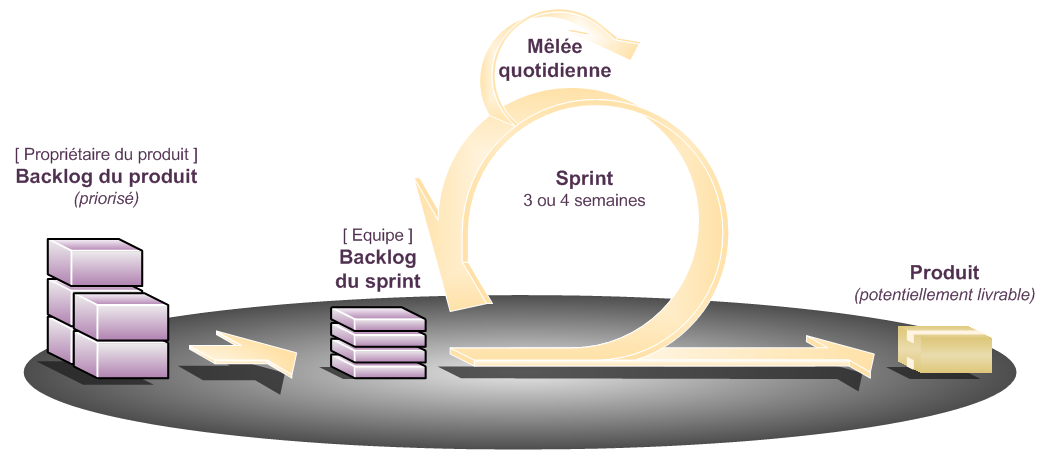
\includegraphics[width=5.0in]{scrum}
    \caption{Principe de la méthode Scrum}
    \label{Scrum}
\end{figure}
\section{Conclusion}
Dans ce chapitre, nous avons présenté le contexte organisationnel du stage afin de prendre une idée claire et précise sur les circonstances de son déroulements, ainsi la cadre contextuel et problématique relative à notre projet.


Nous passerons, dans le prochain chapitre à la présentation d’une solution existante, énumération des critiques et de la solution proposée.

\chapter{ÉTUDE PRÉLIMINAIRE}
\vspace*{3cm}
Afin d'atteindre les objectifs de notre projet, nous allons élaborer une étude préalable. Dans une première partie, nous introduisons les concepts fondamentaux permettant de situer le sujet dans son contexte. Dans une deuxième partie, nous présentons une étude de l'existant et des différents moyens mis à notre disposition pour décortiquer les fonctionnalités déjà développées et surtout de mettre en relief leurs limites afin de dégager une solution.
\pagebreak

\section{Étude de l’existant}
L’utilisation des tablettes pour commercialisation professionnel est trop nouveau, donc pratiquement il n’existe qu’une seule solution "MI Cegedim" qui domine le domaine médical.

\subsection{Étude de MI Cegedim}

MI Cegedim est une plateforme cloud composée par un site web et une application IPAD.

Le site web permet de uploader des présentations en format ZIP qui contient des page web, le site web permet aussi de les mettre à jour et les affecter à des les commerciaux. L’application IPAD permet au personnel de se connecter pour télécharger, mettre à jour et visualiser les présentations qui lui sont associées.

\begin{figure}[H]
    \centering
    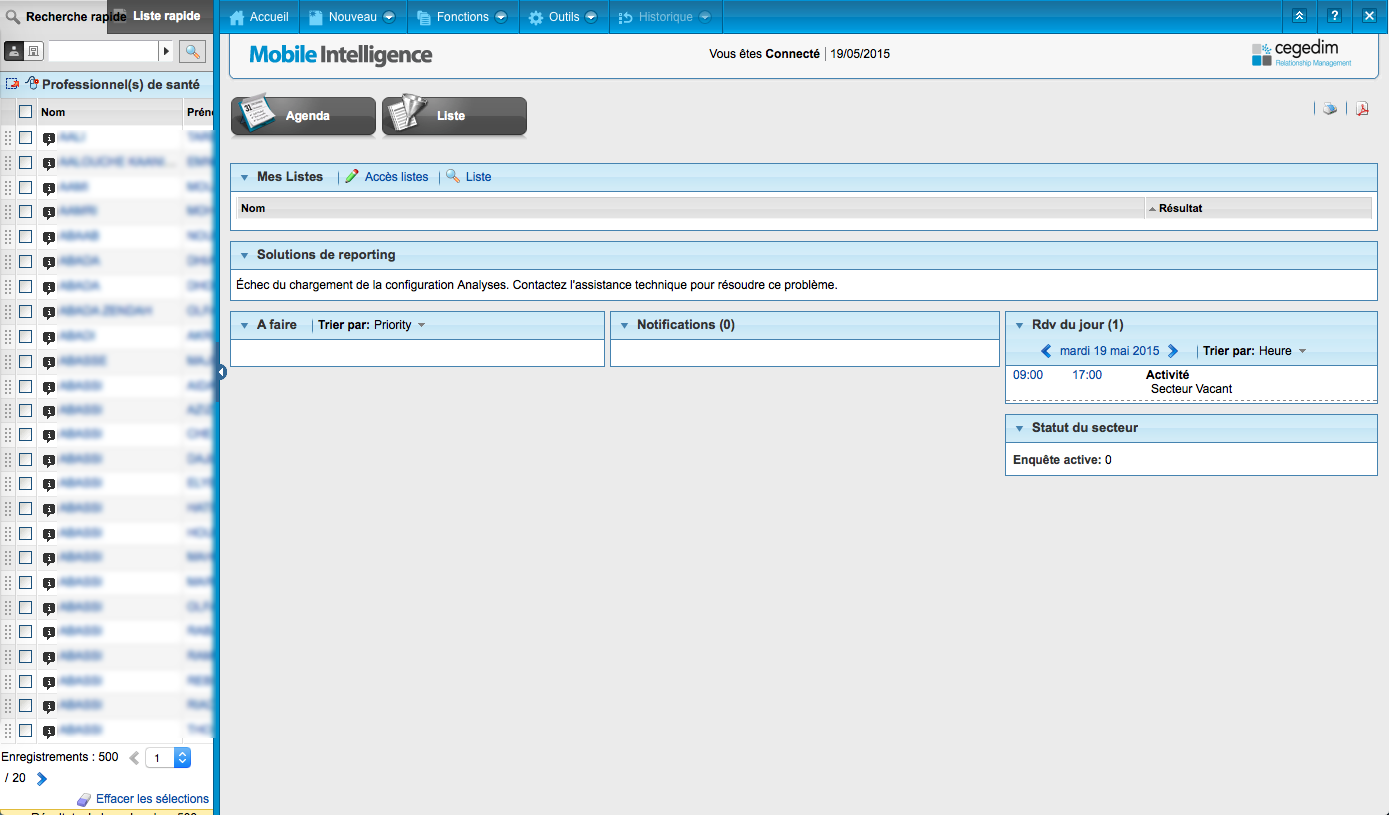
\includegraphics[width=5.5in]{cegedim/web1}
    \caption{Page d'accueil de MI Cegedim}
    \label{Scrum}
\end{figure}

\begin{figure}[H]
    \centering
    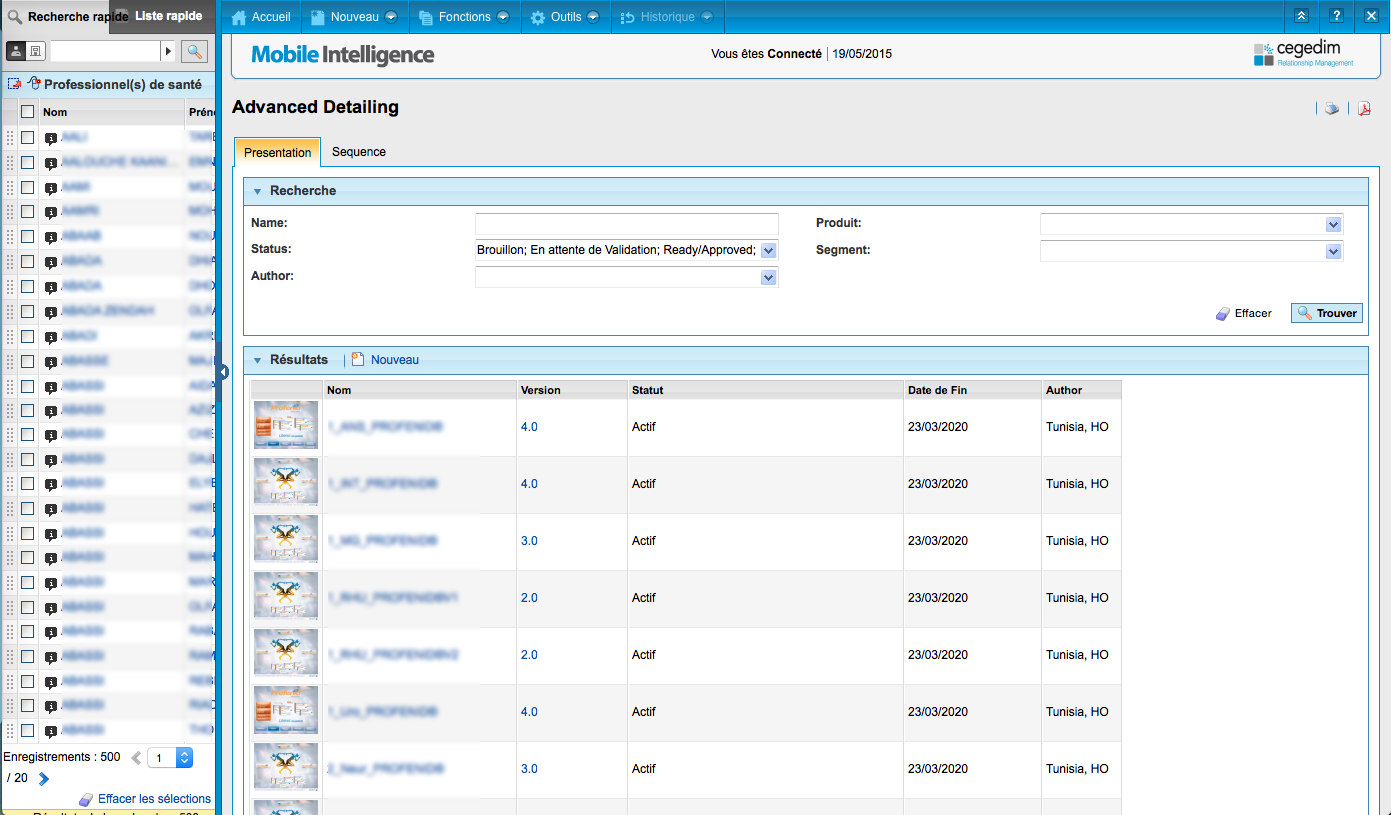
\includegraphics[width=5.5in]{cegedim/web2}
    \caption{Page de liste des présentations de MI Cegedim}
    \label{Scrum}
\end{figure}

\begin{figure}[H]
    \centering
    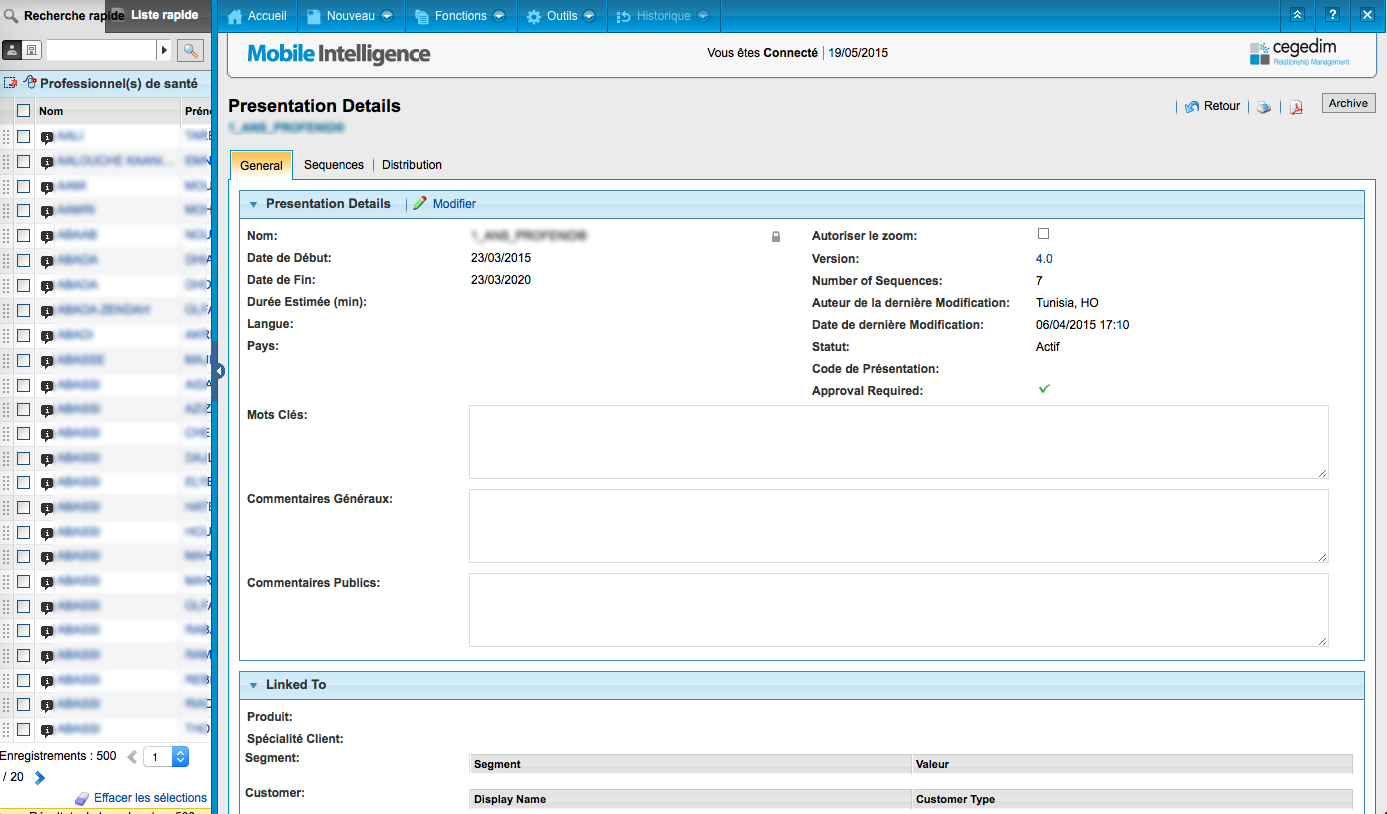
\includegraphics[width=5.5in]{cegedim/web3}
    \caption{Page d'une présentation de MI Cegedim}
    \label{Scrum}
\end{figure}

\begin{figure}[H]
    \centering
    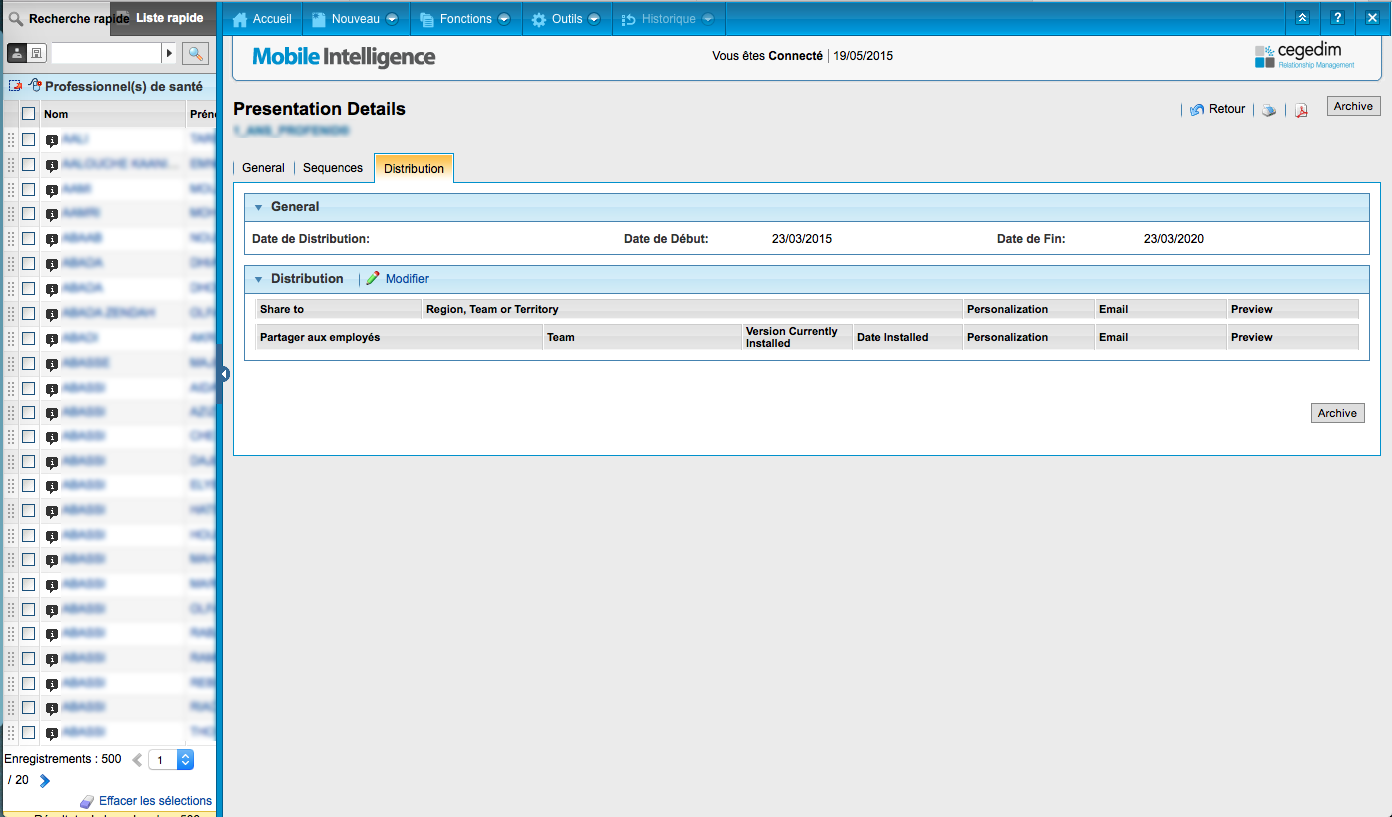
\includegraphics[width=5.5in]{cegedim/web4}
    \caption{Page de distribution de la présentation de MI Cegedim}
    \label{Scrum}
\end{figure}

\begin{figure}[H]
    \centering
    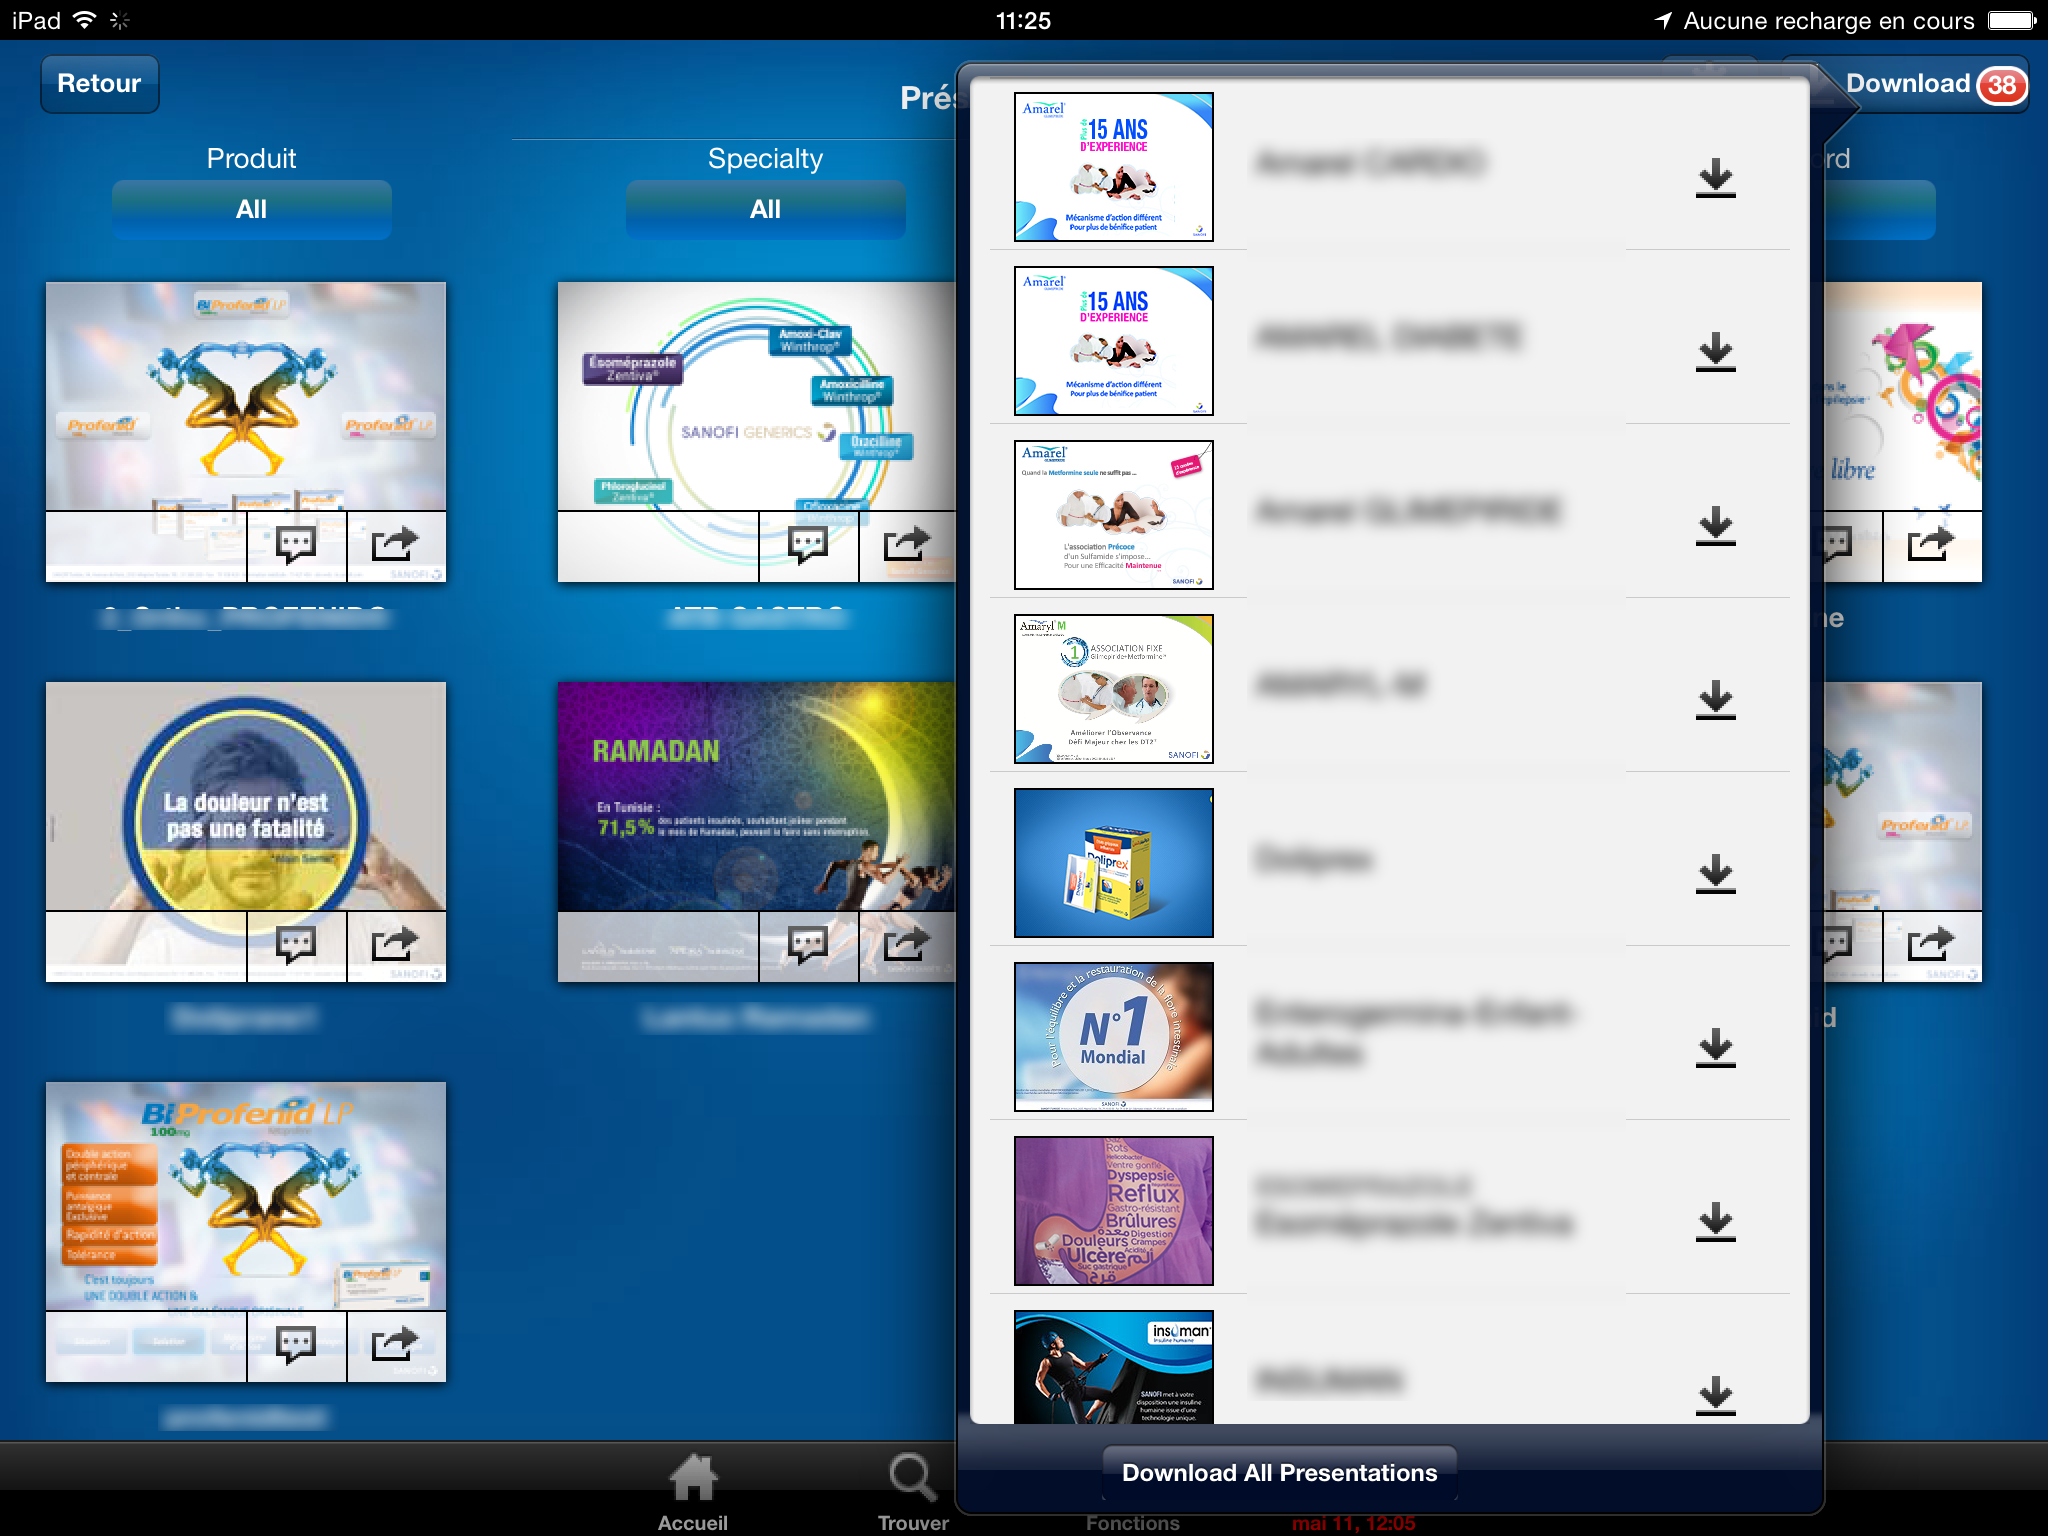
\includegraphics[width=5.5in]{cegedim/app2}
    \caption{Application mobile MI Cegedim}
    \label{Scrum}
\end{figure}

\subsubsection{Avantages}
\begin{itemize}
  \item Le site web offre un gestions totale pour les présentations et les personnels.
  \item Un système de validation.
  \item Héritage des utilisateurs et rôles.
\end{itemize}
\subsubsection{Inconvénients}
\begin{itemize}
    \item Le site web est trop complexe pour l’utiliser.
    \item Le site web est trop lent.
    \item L’ajout et la mise à jour des présentations prend beaucoup de temps pour être effectués.
    \item L’application iPad prend beaucoup temps pour l’exécution pour la première fois.
    \item L’application iPad se plante beaucoup ce qui va mener à réinstaller l’application.
    \item Le téléchargement du présentation dans l’application iPad prend beaucoup du temps.
    \item L’application iPad marche seulement avec connexion internet.
    \item La seule plateforme mobile supporté est iOS pour IPAD.
\end{itemize}
\section{Solution proposée}
En détaillant la problématique et en étudiant la solution existante on peut maintenant énoncer les objectifs à atteindre durant ce projet.

Notre solution consiste à concevoir et réaliser une plateforme de gestion des présentations orientées pour le secteur professionnel(pour les sociétés).

D’un point de vue fonctionnel et pratique, notre plateforme est composée de deux parties :
\begin{itemize}
\item Un site web qui permet une gestion totale des présentations tel que la possibilité d'uploader et de mettre à jour. Il permet aussi de gérer le personnel qui a accès aux présentations. Le site nous offre la possibilité de créer des groupes de personnel ainsi que de visualiser des statistiques.
\item Une application mobile qui permet aux personnels de se connecter et de télécharger, mettre à jour et visualiser les présentations permises. L’application a le pouvoir de collecter des statistiques et de les envoyer au site web.
\end{itemize}
\section{Conclusion}
Dans ce chapitre, nous avons passé en revue la solution existante en mettant l’accent sur ses limites.


Ce qui prépare le terrain à developper les besoins fonctionnels et non fonctionnels, ainsi que les acteurs de notre solution que nous proposons dans le chapitre suivant.
\chapter{Analyse et spécification des besoins}
\vspace*{3cm}
Ce chapitre présente l'étape analytique durant laquelle nous allons recenser et factoriser les besoins communs aux utilisateurs du service d’authentification. Ceci, allié à l’étude menée au cours du premier chapitre, nous permettra d’obtenir l'ossature du projet que nous formaliserons ensuite sous forme de diagrammes UML.
\pagebreak
\section{Les acteurs du système}
Les utilisateurs invoqués dans le système et que nous chercherons à satisfaire les besoins sont :
\begin{description}
    \item [L’administrateur] : il est responsable de la gestion du présentation, du personnels et du groupe.
    \item [Le personnel] : on désigne par personnel les utilisateurs qui vont visualiser les présentations sur l'application mobile.
\end{description}
\section{Détermination des besoins}
L’analyse du sujet a permis de dégager les fonctionnalités qui seront mises à la disposition des acteurs. Les besoins ainsi dégagés sont classés en besoins fonctionnels et besoins non fonctionnels.
\subsection{Spécification des besoins fonctionnels}
\subsubsection{besoins fonctionnels du plateforme web}
\begin{description}
\item [Gestion de présentation ]: l'administrateur peut ajouter, supprimer, éditer et mettre à jour les présentations, et peut aussi associer des présentations à aux personnels ou à des groupes.

\item [Gestion du personnel] : l'administrateur peut ajouter, modifier et supprimer du personnel.

\item [Gestion de groupes] : un groupe est un ensemble des personnels groupés dans un seule entité peut être créer, modifier ou supprimer par l'administrateur.

\item [Statistique] : la plateforme web permet d’afficher des statistiques collectés et calculés depuis l’application mobile, les statistiques consistent aux nombre de vues par jour, les délais dans chaque page et même les réponses aux questions par présentation.
\end{description}
\subsubsection{besoins fonctionnels du applications mobile}

\begin{description}
\item [Visualisation des présentations] : un personnel peut se connecter et télécharger, mettre à jour et visualiser les présentations qui lui sont associeés.

\item [Statistique] : l’application mobile permet automatiquement de collecter des statistiques et des informations d’une manière autonome, et les envoyer aux serveur.

\item \textbf{Mode déconnecté} : l’application mobile doit fonctionner sans connexion internet, offrant la possibilité aux personnel ,qui utilisent l’application avant de se connecter et visualiser les présentations locales, et même de collecter les statistiques pour l’envoyer dés qu'une connexion internet soit disponible.
\end{description}
\subsection{Spécification des besoins non fonctionnels}
\begin{description}
\item [Extensibilité]
il faut utiliser une architecture évolutive, qui permet la facilité d’ajouter d’autres fonctionnalités.
\item [Sécurité]
la plateforme vise des utilisateurs dans le domaine professionnel donc il faut garantir la sécurité et la confidentialité des leurs informations.
\item [Temps de réponse]
les tâches doivent s’exécuter dans un temps raisonnable, pour garantir une expérience fluide et rapide.
\item [Disponibilité]
la plateforme doit être toujours disponible.
\item [Simplicité]
la plateforme doit offrir une expérience d’utilisation simple et facile.
\end{description}
\section{Spécifications Fonctionnelles Détaillées}
La conception détaillée d’un projet vise à expliquer en détail l’organisation et la répartition des tâches entre les modules et les objets constituants le projet afin de préparer la phase de réalisation. Elle a pour but d’expliquer les solutions choisies afin de mettre en place les modules et les différents scénarios qui seront exécutés par l'application. En outre, cette phase englobe aussi la préparation des plans de tests unitaires de chaque module qui permettent de voir si le module répond aux spécifications du projet ou non.
\subsection{Diagramme global des Cas d’utilisation}
\subsubsection{Diagramme Global des Cas d’utilisation du la plateforme web}

\begin{figure}[H]
    \centering
    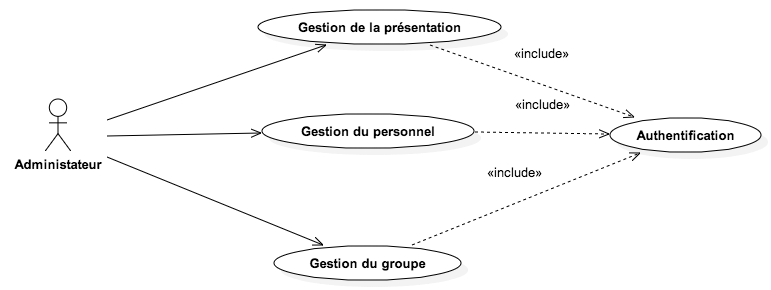
\includegraphics[width=5.0in]{UseCaseDiagramWeb}
    \caption{Diagramme de cas utilisation du plateforme web}
    \label{UseCaseDiagramWeb}
\end{figure}

\paragraph{Description textuelle du cas "Gestion de la présentation"}

L'administrateur peut ajouter, éditer, supprimer et mettre à jour les présentations.
Pour chaque présentation il peut aussi associer du personnel.
Il peut aussi visualiser les statistiques de chaque présentation.
\paragraph{Description textuelle de cas "Gestion du personnel"}
L'administrateur peut ajouter, modifier et supprimer du personnel.
\paragraph{Description textuelle de cas "Gestion du groupe"}
L'administrateur peut créer, modifier et supprimer les groupes.


\subsubsection{Diagramme Global des Cas d’utilisation de l'application mobile}

\begin{figure}[H]
    \centering
    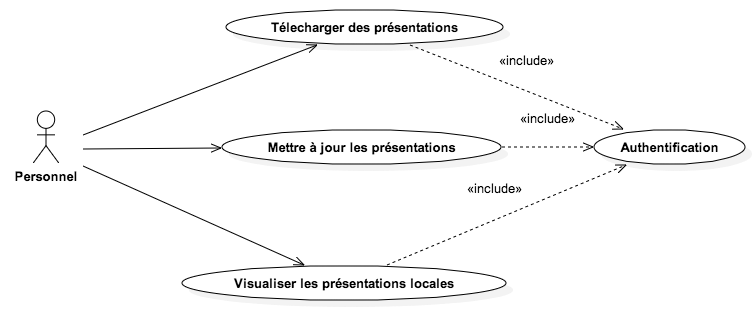
\includegraphics[width=5.0in]{UseCaseDiagramApp}
    \caption{Diagramme de cas utilisation du application mobile}
    \label{UseCaseDiagramWeb}
\end{figure}
\paragraph{Description textuelle de cas "Télécharger présentations"}

Le personnel peut télécharger les présentations associées à lui.
Les présentations téléchargées seront toujours disponibles et accessibles par les autres personnels qui ont droit.
\paragraph{Description textuelle de cas "Mettre à jour les présentations"}
Le personnel peut mettre à jour les présentations locaux quand des mise à jour sont disponibles
\paragraph{Description textuelle de cas "Visualiser les présentations locales"}
Le personnel peut visualiser les présentation locales.
\subsection{Diagramme Détaillé des Cas d’utilisation}
\subsubsection{plateforme web}
\paragraph{Gestion de présentations}

\begin{description}
  \item[Ajouter une présentation] permet d'uploader une nouvelle présentation, elle est sous format ZIP qui contient nécessairement deux fichiers "index.html" et "thumb.jpg". Avec le fichier ZIP l'administrateur doit entrer aussi le nom et la description de la présentation.
  \item[Editer une présentation] permet de modifier les informations d'une présentation comme nom et description.
  \item[Mettre à jour une présentation] permet d'uploader une nouvelle version du fichier ZIP de la présentation, qui va incrémenter le numéro de la version du présentation.
    \item[Supprimer une présentation] permet de supprimer une présentation définitivement
      \item[Associer du personnel à une présentation] permet d'associer des personnels à une présentation, qui leur permet de les visualiser.
      \item[Visualiser les statistiques d'une présentation] permet aux administrateur de visualiser les statistiques collectés par l'application mobile.
\end{description}
\begin{figure}[H]
    \centering
    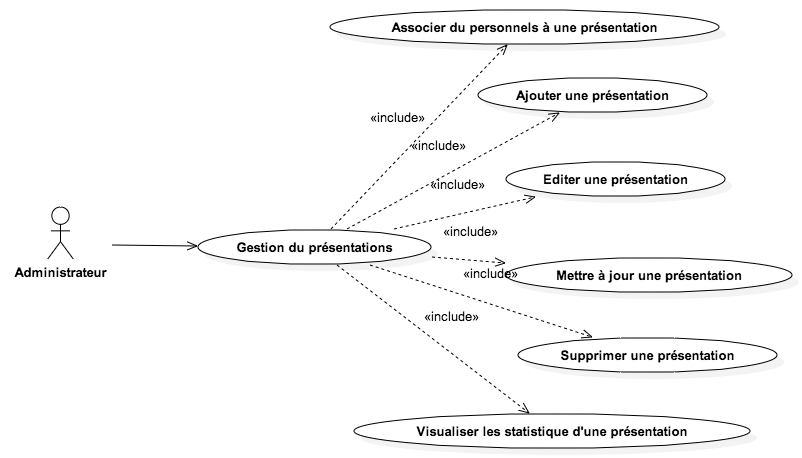
\includegraphics[width=5.0in]{UseCaseGestionPresentations}
    \caption{Diagramme de cas utilisation de gestion de présentations dans plateforme web}
    \label{UseCaseDiagramWeb}
\end{figure}

\paragraph{Gestion du personnel}
\begin{description}
  \item[Ajouter un personnel] permet d'ajouter un personnel à l'application mobile.
    \item[Modifier un personnel] permet de modifier les informations d'un personnel.
    \item[Supprimer un personnel] permet de supprimer un utilisateur de l'application mobile.
\end{description}
\begin{figure}[H]
    \centering
    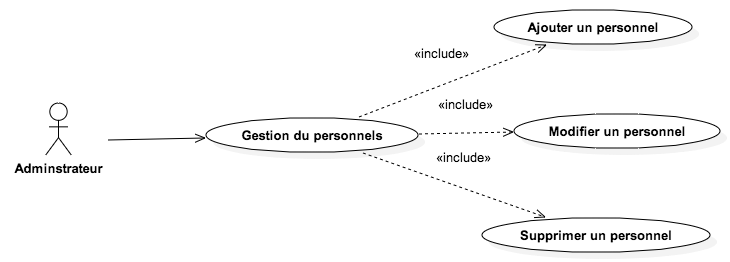
\includegraphics[width=5.0in]{UseCaseGestionPersonnel}
    \caption{Diagramme de cas utilisation du Gestion de présentations dans la plateforme web.}
    \label{UseCaseDiagramWeb}
\end{figure}

\paragraph{Gestion du groupe}
\begin{description}
    \item[Créer un groupe] l'administrateur peut créer un groupe en donnant son nom et description.
    \item[Supprimer un groupe] l'administrateur peut supprimer un groupe définitivement.
    \item[Ajouter un personnel] l'administrateur peut associer des personnels à un groupe.
    \item[Supprimer un personnel] l'administrateur peut dé-associer des personnels d'un groupe.
\end{description}

\begin{figure}[H]
    \centering
    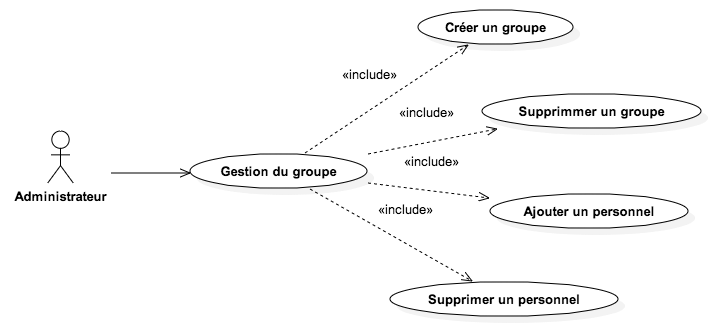
\includegraphics[width=5.0in]{UseCaseGestionGroupe}
    \caption{Diagramme de cas utilisation du Gestion de groupe dans la plateforme web}
    \label{UseCaseDiagramWeb}
\end{figure}



\section{Conclusion}
Ce chapitre nous avons permis de couvrir les différents besoins fonctionnels et non fonctionnels des acteurs de notre système. Nous avons fourni une analyse plus détaillée de ces besoins grâce à l’ensemble des diagrammes de cas d’utilisation. La spécification des besoins étant établie, nous essayerons dans le chapitre suivant de concevoir clairement l’architecture de notre service.
\chapter{Étude conceptuelle}
\vspace*{3cm}
Après avoir présenté dans le chapitre précédent la phase de spécification des besoins et dégager les principales fonctions de la solution à mettre en œuvre, nous présentons dans ce chapitre la phase de conception. Cette phase nécessite la mise en place d’un modèle sur lequel nous allons s’appuyer dans l’implémentation.
Nous commençons par présenter la conception générale de notre plateforme à travers son architecture générale et son diagramme de composants. Nous présentons par la suite la conception détaillée de notre base de données suivie par la conception détaillée de notre plateforme via les diagrammes de classes, séquences et activités reflétant les aspects statiques et dynamiques.
\pagebreak
\section{Conception générale}
Nous abordons, dans cette section, l’aspect général de notre plateforme à travers la présentation de son architecture générale et son diagramme de composants.
\subsection{Architecture générale de la plateforme}
Nous avons adopté dans notre plateforme une architecture 3 tiers dont les fonctions sont distribuées sur deux systèmes clients (Application mobile et Navigateur web), un serveur web et un serveur de la base de données MySQL pour la partie Web et Mobile.
Toute communication entre Application mobile et le serveur web utilise l'architecture REST[4] avec une méthode d'authentification JWT (Json Web Token)[5].
Pour la version du production de la plateforme toutes les communications entre le serveur web et les clients mobile et web utilisent le protocole HTTPS.
La figure 4.1 illustre l'architecture.
\begin{figure}[H]
    \centering
    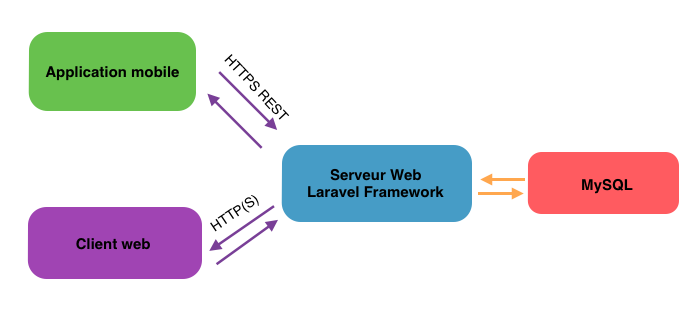
\includegraphics[width=5.0in]{archi}
    \caption{Architecture de Plateforme globale}
    \label{diagdeploit}
\end{figure}

\subsection{Architecture de présentation}
Toutes les présentations sont développées avec HTML5 (avec CSS3 et Javascript[3]), qui offre des infinités de possibilité d'animations et interactions.

Chaque présentation est un fichier \textbf{Zip} qui contient deux fichiers nécessaires :
\begin{description}
\item[index.html] la page principale de présentation qui va être affichée en premier sur l'application mobile.
\item[thumb.jpg] l'image qui va représenter la présentation dans l'affichage dans le site web ou dans l'application mobile.
\end{description}

\begin{figure}[H]
    \centering
    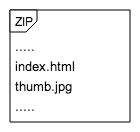
\includegraphics[width=2.0in]{zippresentation}
    \caption{Architecture de présentation}
    \label{diagdeploit}
\end{figure}

\subsubsection{API et communication entre présentation et application mobile}
L'application mobile fournit à chaque présentation un ensemble des fonctionnalités accessibles par l'API javascript[3].
\begin{figure}[H]
    \centering
    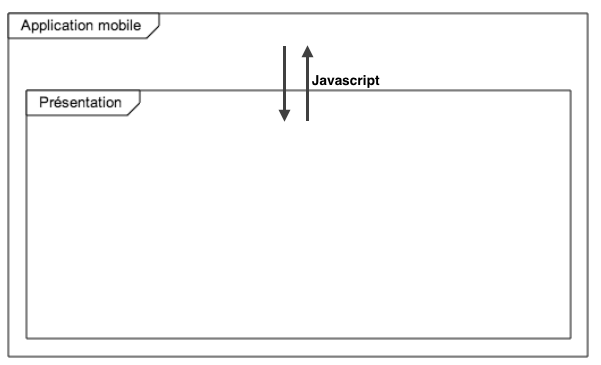
\includegraphics[width=4.0in]{apipresentation}
    \caption{Architecture de communication entre l'application mobile et la présentation}
    \label{diagdeploit}
\end{figure}


\begin{table}[H]
\centering
\begin{tabular}{ | p{3cm} | p{5cm} | p{5cm} | }
 \hline
 Nom de la méthode & Paramètres & Description \\
 \hline
 Délai page  & 
  \begin{description}
 \item[Délais] tableau
 \end{description}
 & Permet d'envoyer les délais de chaque page à la plateforme web\\
  \hline
 Question  & 
 \begin{description}
 \item[Question] chaine
 \item[Réponse] tableau
 \item[index de réponse] entier
 \end{description}
 & Permet d'envoyer les réponses des questions à la plateforme web\\
\hline
\end{tabular}
\caption{Tableau des méthodes accessible par présentation}
\label{table:1}
\end{table}


\subsection{Diagramme de déploiement}
Le diagramme de déploiement permet d'illustrer l'architecture physique du système et de montrer la relation entre ses différentes composantes. La figure 4.4 présente le diagramme de déploiement de notre plateforme.

\begin{figure}[H]
    \centering
    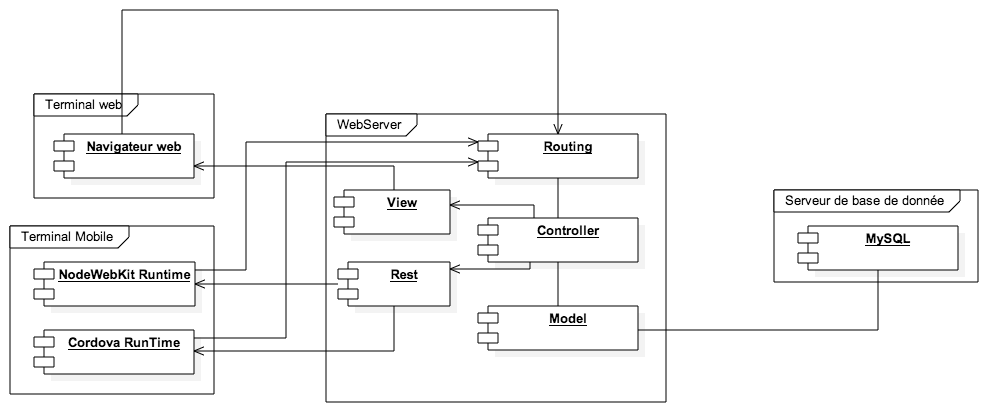
\includegraphics[width=6.0in]{DeploymentDiagram}
    \caption{Diagramme de déploiement}
    \label{diagdeploit}
\end{figure}
\pagebreak
\subsection{Diagramme de classes}
Le diagramme de classe, schématisé dans la figure 4.5, fournit un aperçu sur les différentes entités de la solution de gestion des présentations.
\begin{figure}[H]
    \centering
    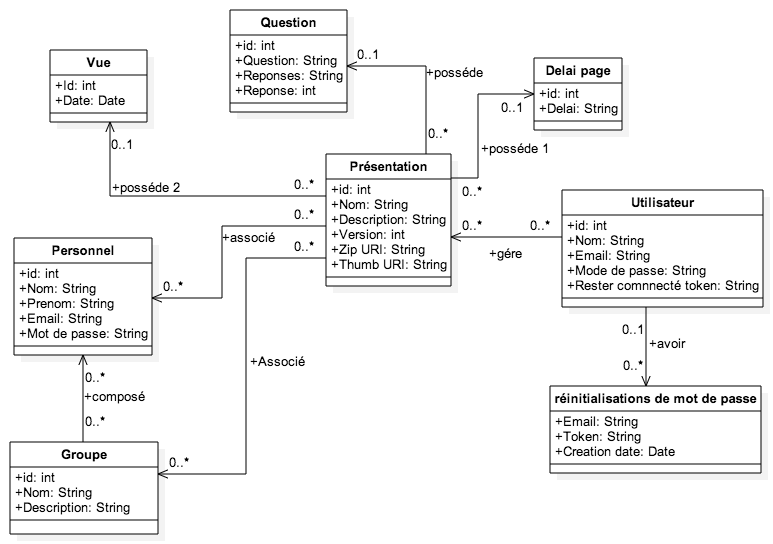
\includegraphics[width=6.0in]{diagclass}
    \caption{Diagramme de classe}
    \label{diagclass}
\end{figure}
\pagebreak
Chaque entité de de diagramme de classes est décrite dans le tableau 4.2.

\begin{table}[H]
{\renewcommand{\arraystretch}{3}%
\begin{tabular}{ | p{4cm} | p{10cm} | }
 \hline
 \textbf{Nom de l'entité} & Description \\
 \hline
 \textbf{Présentation}
 &  Classe entité qui représente tous les présentations ajoutées dans la plateforme.\\
  \hline
 \textbf{Utilisateur}
 & Classe entité qui décrit les utilisateurs qui vont utiliser le site web.\\
\hline
 \textbf{Personnel}
 & Classe entité symbolise les utilisateurs qui vont utiliser l’application mobile.\\
\hline
 \textbf{Groupe}
 & Classe entité qui permet de grouper un ensemble de personnel dans une seule entité.\\
\hline
 \textbf{Question}
 & Classe entité qui représente une question d’une présentation, avec ces réponses.\\
\hline
 \textbf{Vue}
 & Classe entité qui symbolise les dates de visualisation d’une présentation.\\
\hline
 \textbf{Délai page}
 & Classe entité qui contient les délais temporaires de chaque page dans une présentation.\\
\hline
 \textbf{Réinitialisations de mot de passe}
 & Classe entité qui représente les jetons de réinitialisations de mot de passe.\\
\hline
\end{tabular}} \quad
\caption{Tableau de description des entités de diagramme de classes}
\label{table:1}
\end{table}

\vspace{15mm}


\subsection{Diagramme de séquence}
\subsubsection{Site web}

\begin{figure}[H]
    \centering
    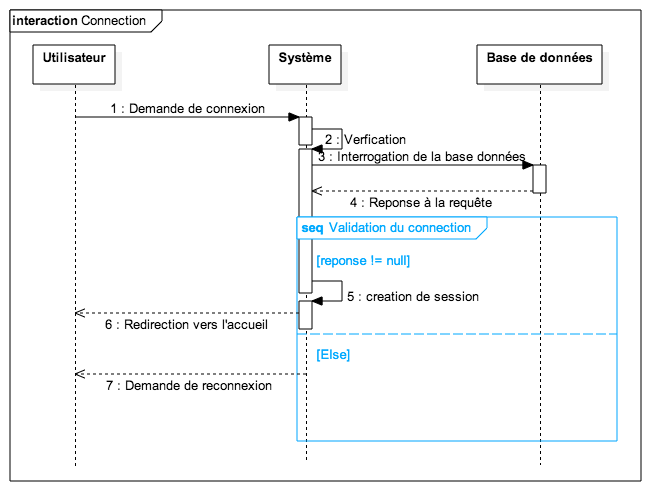
\includegraphics[width=6in]{diagsequenceloginweb.png}
    \caption{Diagramme de séquence de connexion site web}
    \label{diagdeploit}
\end{figure}

\vspace{20cm}

\begin{figure}[H]
    \centering
    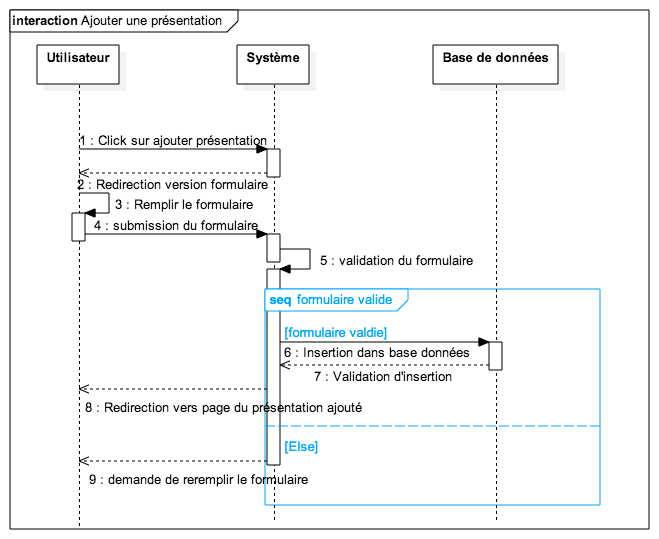
\includegraphics[width=6in]{diagsequenceajoutepres}
    \caption{Diagramme de séquence d'ajoute de présentation}
    \label{diagdeploit}
\end{figure}


Le diagramme d'ajout du personnel ou du groupe est identique à celui d'ajout d'une présentation.

\vspace{15cm}

\subsubsection{Application mobile}


\begin{figure}[H]
    \centering
    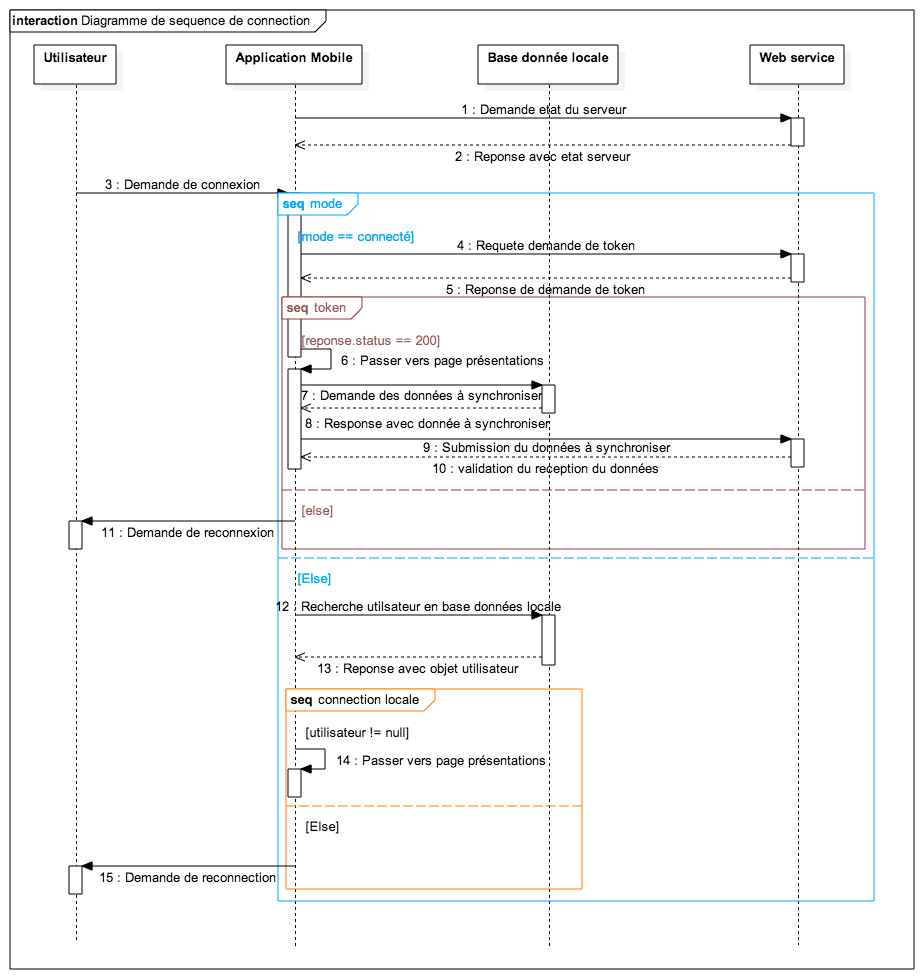
\includegraphics[width=6in]{diagsequenceloginmobile}
    \caption{Diagramme de séquence de connexion application mobile}
    \label{diagdeploit}
\end{figure}
L'application mobile doit être toujours accessible dans d’absence de connexion internet ou maintenance du site web.


Dans le cas où le site web est injoignable, la validation des identifiants se fait par la base donnée locale.




Sinon si tout est à l’ordre, la connexion se fait par un service web REST sécurisé par la méthode authentification JWT (JSON WEB TOKEN)[1] qui va générer un jeton temporaire et qui va être utilisé dans toutes les prochaines communications entre l’application mobile et le site web.

\section{Conclusion}
A travers ce chapitre, nous avon mis en oeuvre la faisabilité de notre framework. En premier lieu, nous avons présenté l’architecture globale de notre projet. Ensuite, nous avons abordé la conception globale de notre solution à travers la présentation du diagramme de déploiement ainsi que les différents diagrammes de classe.


Enfin, nous avons présenté une vue dynamique de la plateforme à travers les différents diagrammes de séquence que nous avons jugé nécessaires pour l’explication du fonctionnement de notre projet.


Après avoir spécifié nos besoins et nos objectifs et entamé notre étude conceptuelle, nous allons voir en détail, dans le prochain chapitre, une description des outils et frameworks qui nous ont permis de réaliser et intégrer notre plateforme.
\chapter{Mise en œuvre et Réalisation}
\vspace*{3cm}
Une des étapes de la vie d'un projet, aussi importante que la conception, est l'implémentation. Cette étape constitue la phase d'achèvement et d'aboutissement du projet. Pour l'accomplir avec succès, il faut savoir utiliser les outils nécessaires et adéquats. Ce chapitre constitue le dernier volet de ce rapport. Pour se faire, nous allons commencer par la présentation de l'environnement matériel et logiciel sur lesquels nous avons réalisé notre travail, tout en justifiant les différents choix technologiques effectués. Ensuite, nous allons présenter notre travail à travers quelques interfaces graphiques.
\pagebreak
\section{Environnement de travail}
Dans ce qui suit, nous présentons l’environnement matériel mis à la disposition du présent projet ainsi que l’environnement logiciel qui a permis l’aboutissement de la mise en œuvre du logiciel.

\subsection{Environnement de développement}
Cette partie est consacrée à la présentation des différents outils composant notre environnement de développement.
\subsubsection{Système d'exploitation du développement}
Le développement du projet a été mené sur OsX 10.10 avec un custom Shell \textbf{ZSH} avec un framework OH-MY-ZSH.

Le système contient aussi un gestionnaire de package \textbf{BREW}.
La version de PHP utilisé \textbf{PHP 5.5.22, Zend Engine v2.5.0} avec extension \textbf{Xdebug}.
\subsubsection{IDE}
\begin{description}
\item[IntelliJ IDEA] : classé comme l’un des plus intelligent IDA dans le monde grâce à sont support à plusieur frameworks marquants comme Spring, GWT, Grails, Play et AngularJS.
Il comprend un ensemble étonnant d'outils qui fonctionnent de la boîte-à-support pour: Maven, Gradle et STS; intégration avec Git, SVN, Mercurial; base de données intégrée Outils, etc.
\item[PhpStorme] : Appartient à la famille de IntelliJ IDEA, il offre les mêmes fonctionnalités avec un support total pour le developpement web avec ses principaux outils et frameworks.
\end{description}
\subsubsection{Outil}
\begin{description}
\item[GIT] : est un système de contrôle de révision distribué avec un accent sur la vitesse, l'intégrité des données, et le soutien aux distribués. Git a été initialement conçu et développé par Linus Torvalds pour le développement du noyau Linux en 2005, et est depuis devenu le plus largement adopté comme système de contrôle de versions pour le développement de logiciels.
\item[NPM] : est un gestionnaire de paquets pour JavaScript. Npm est livré et installé automatiquement avec le environment. NPM traverse la ligne de commandes et gère les dépendances d'une application. Il permet également aux utilisateurs d'installer des applications Node.js, qui sont disponibles sur le registre de NPM.
\item[Gulp] : est outil de build web basé sur les tâches, il permet d'automatiser et d'accéler la développement, les tâches les plus utilisées sont la compilation de Sass, la minimisation, la fusion des fichiers .js et .css et la génération d’une version du production.
\item[Bower] [10]:  est un système de gestion des paquets pour la programmation côté client sur le World Wide Web. Il dépend de Node.js et NPM. Il fonctionne avec git et dépôts GitHub.
\item[Composer] : est un gestionnaire de dépendance niveau de l'application pour le langage de programmation PHP qui fournit un format standard pour la gestion des dépendances de logiciels PHP et les librairies nécessaires. Composer est fortement inspiré par «NPM» de Node.js et "bundler" Ruby. 
Composer traverse la ligne de commande et installe les dépendances d'une application. Il permet également aux utilisateurs d'installer des applications PHP qui sont disponibles sur "Packagist" qui est son principal référentiel contenant les packages disponibles. Il fournit également des capacités de chargement automatique pour les bibliothèques aussi spécifique aux informations autoload pour faciliter l'utilisation de code tiers.
\item[YO] [10] : permet l'échafaudage d'une nouvelle application, l'écriture de la configuration de construction (par exemple Gruntfile, Gulpfile) et de tirer dans les tâches de construction pertinentes et gestionnaire de paquetages dépendances (Bower, NPM).
\item[Chrome Developer Tools] : sont un ensemble des outils de création de pages Web et de débogage intégrés dans Google Chrome. Les DevTools fournissent aux développeurs Web un accès en profondeur dans les internes du navigateur et de leur application web. Utilisez les DevTools pour suivre efficacement les problèmes, définissez des points d'arrêt JavaScript, et obtenir des idées pour l'optimisation de code.
\item[StarUML] : est un logiciel opensource. Il s'agit d'une plateforme de modélisation avec le langage UML. Cet outil propose tous les diagrammes nécessaires à une bonne modélisation.
\end{description}

\subsection{Environnement d’exécution}
\subsubsection{Requise pour le serveur web}
\begin{itemize}
\item $Php \geq $5.4

\item Composer
\item Mcrypt PHP Extension
\item OpenSSL PHP Extension
\item Mbstring PHP Extension
\item Tokenizer PHP Extension
\item Json PHP Extension
\item MySQL
\item GIT
\end{itemize}
\subsubsection{Requise pour l'application mobile}
\begin{description}
\item[Cordova Runtime] [7]: $Cordova \geq $5.0.0
Plugins : cordova-plugin-file-transfer, MobileChromeApps-zip, phonegap-hash
\item[NodeWebkit Runtime] [8]: $NWJS \geq $0.12.1
plugins : adm-zip
\end{description}
\subsection{Librairies utilisées}
\subsubsection{Librairies utilisées pour la plateforme web}
\textbf{Laravel}[9] : est basé sur une structure MVC (modèle – vue – contrôleur), mais avec quelques curiosités. Tout d’abord, Laravel se fonde sur des méthodes statiques. Cette manière de fonctionner simplifie la programmation, mais complique un peu la création de ses propres classes et méthodes. La machinerie du cœur du framework est assez complexe avec un système d’injection de dépendances.
Laravel est particulièrement souple. En particulier, le fameux fichier route.php dans lequel on devrait mettre les routes gérant les url, peut contenir à peu près tout. On pourrait créer un site complet en n’utilisant que le fichier route.php. Un autre point inquiétant vient de la documentation de Laravel.
En conclusion, Laravel est un bon framework, efficace, facile, plaisant à utiliser, rapide, avec une faible empreinte mémoire. Il faudra néanmoins faire attention à ne pas abuser de la liberté offerte.


Le choix de ce framework est basé aussi sur son classement par rapport les autres frameworks Php comme illustre les figures 5.1 et 5.2.


\begin{figure}[H]
    \centering
    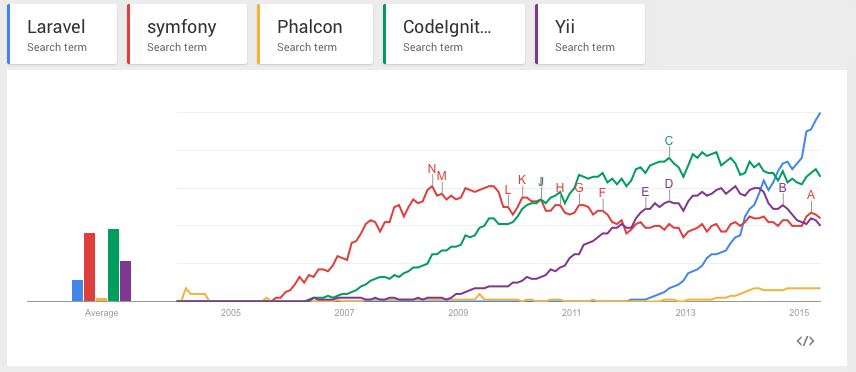
\includegraphics[width=6in]{laravel/laraveltrends}
    \caption{Tendances des frameworks php [12]}
\end{figure}


\begin{figure}[H]
    \centering
    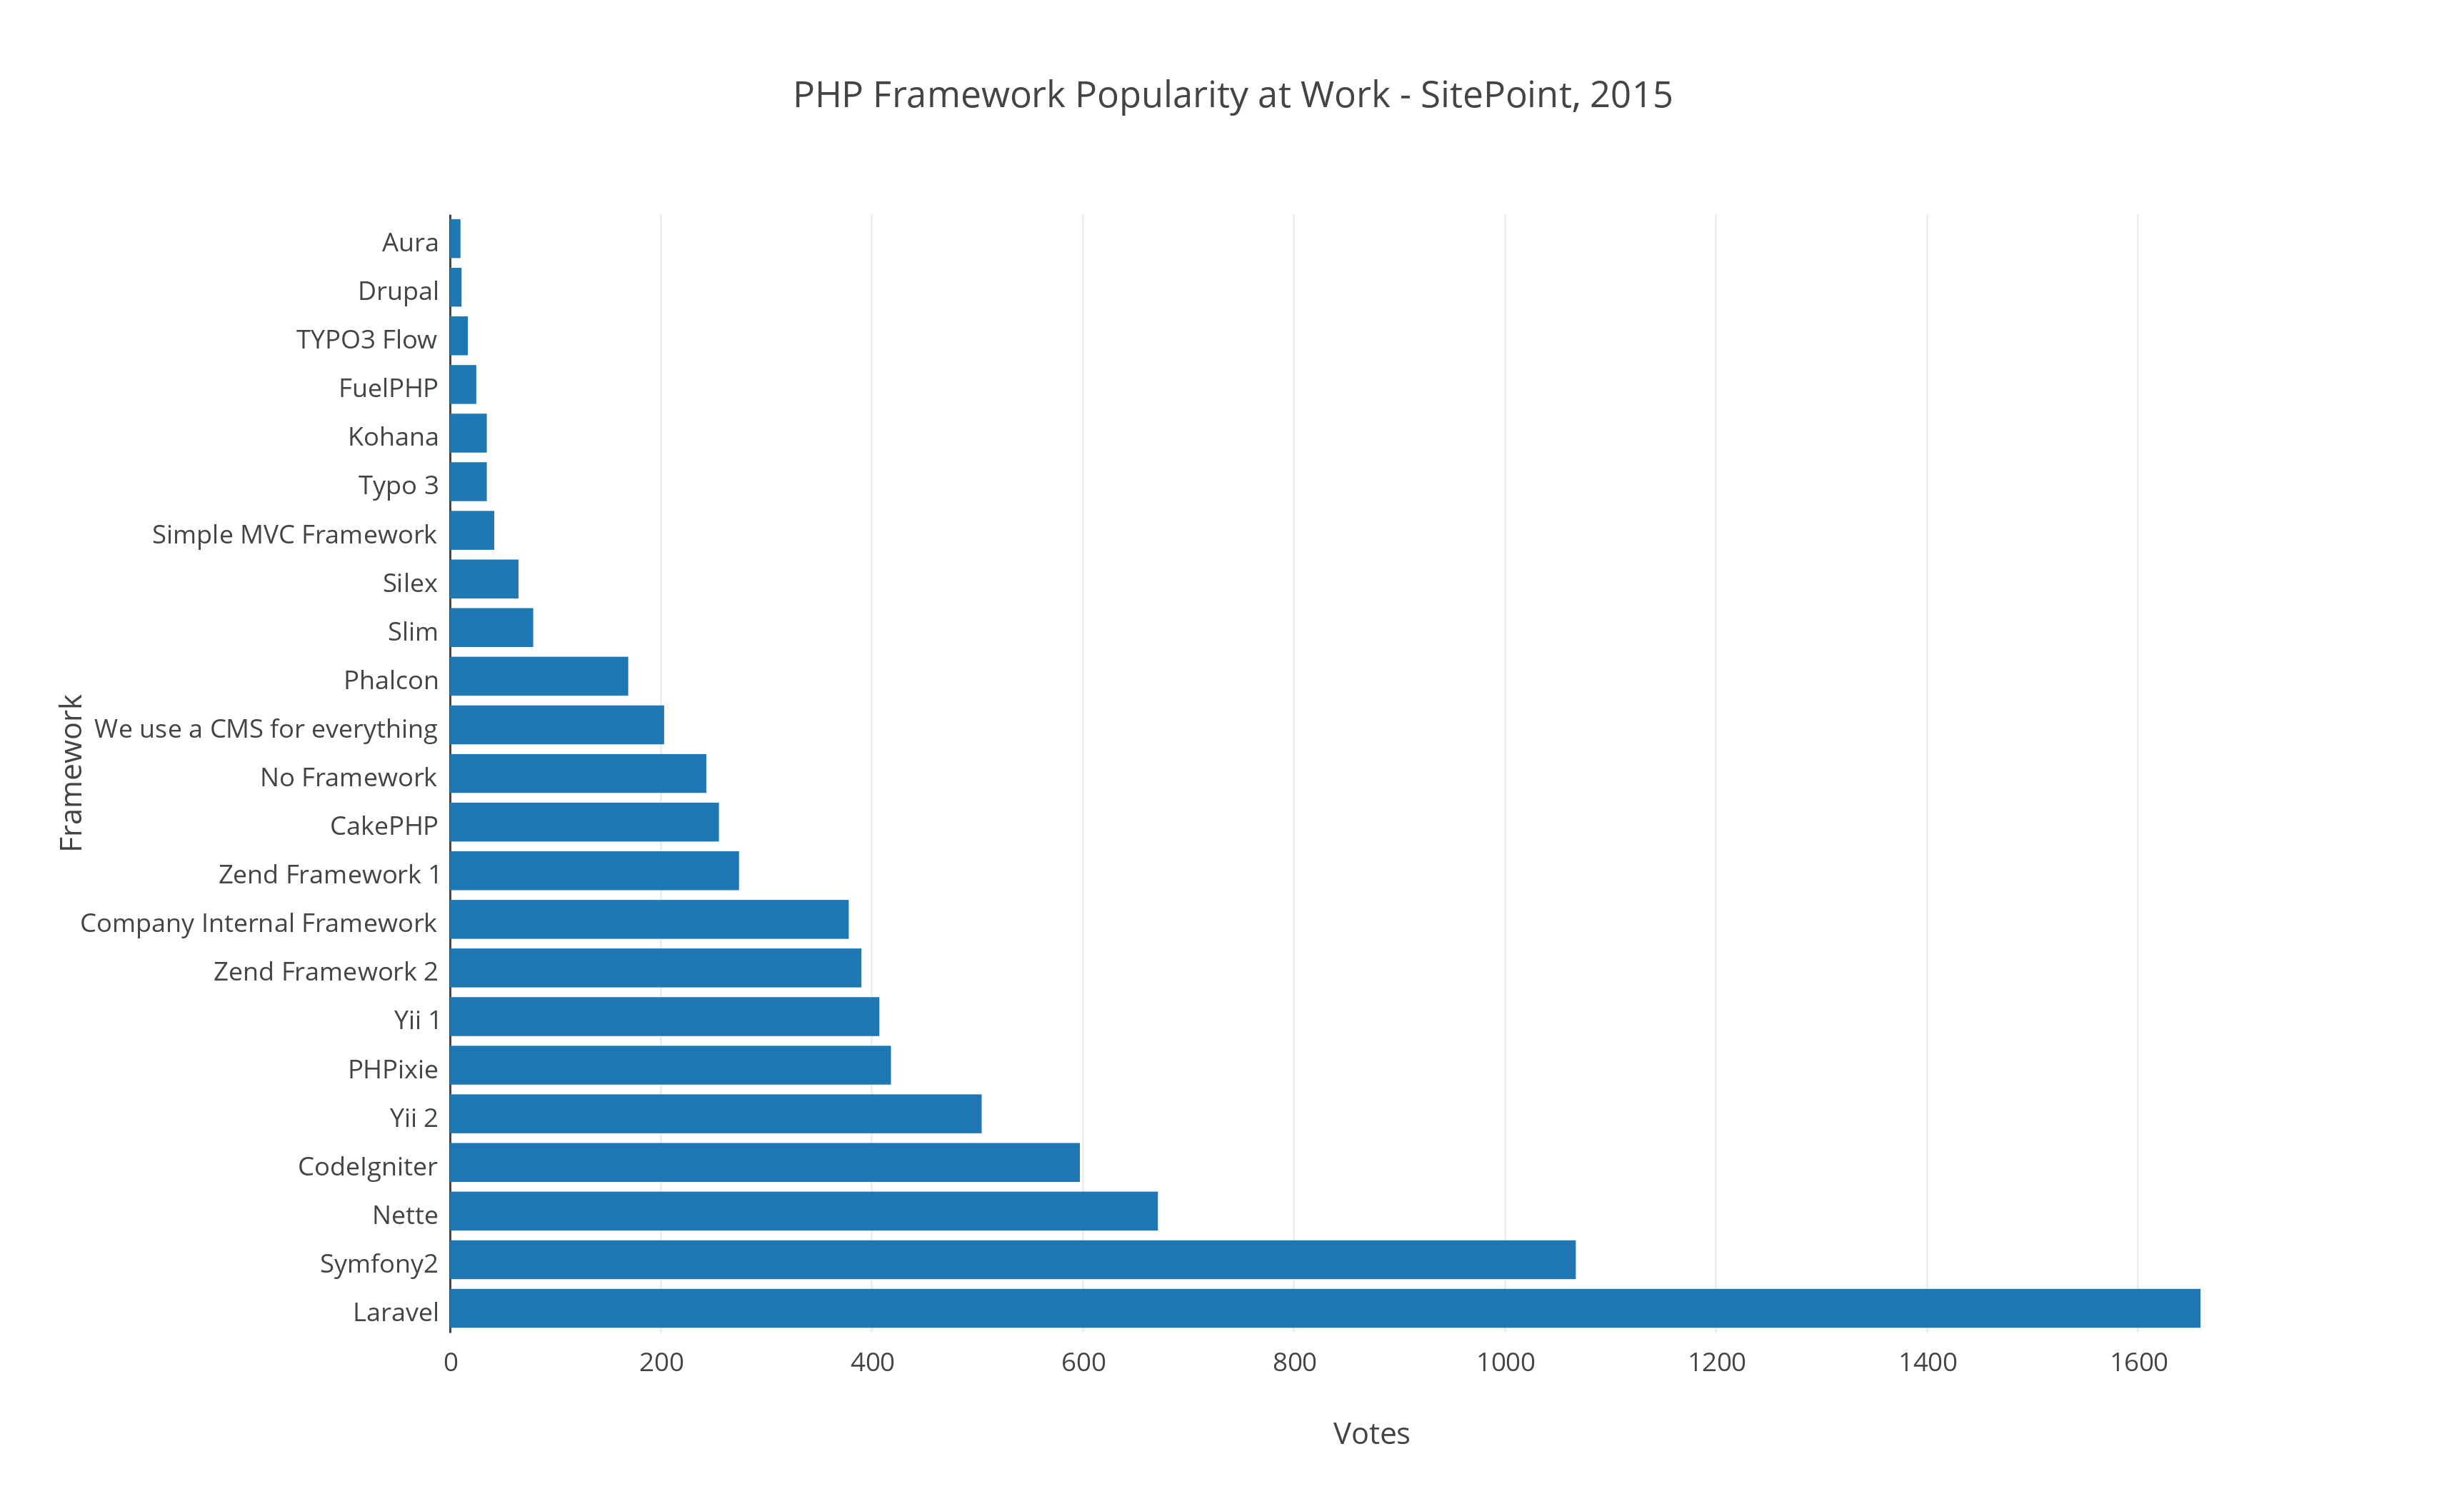
\includegraphics[width=5.5in]{laravel/php_framework_popularity_at_work}
    \caption{La popularité des frameworks php dans le domaine professionnel[13]}
\end{figure}

\subsubsection{Librairies utilisées dans la partie mobile}
\textbf{AngularJS}[2,14] :  est un framework d'applications Web open-source maintenu par Google et une communauté de développeurs et d'entreprises individuelles pour répondre à bon nombre des difficultés rencontrées dans le développement d'applications d'une seule page. Son objectif est de simplifier le développement et l'essai de ces applications en fournissant un cadre pour le modèle-vue-contrôleur côté client (MVC) architecture, avec des composants couramment utilisés dans des applications Internet riches.


Et comme illustre la figure 5.3, on individualise que Angular JS domine la tendance de recherche. 
\begin{figure}[H]
    \centering
    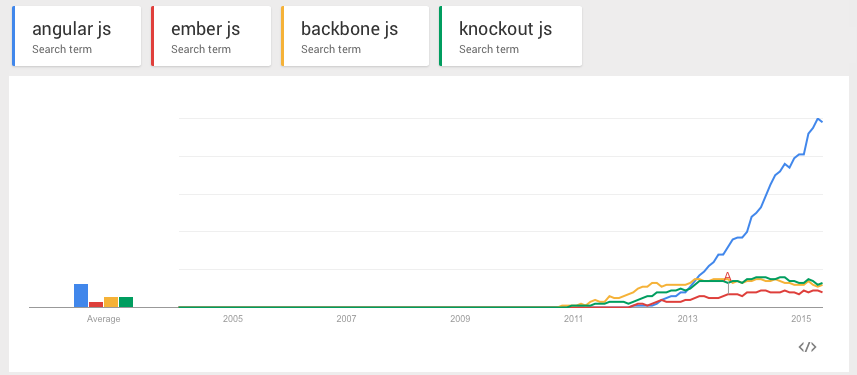
\includegraphics[width=6in]{angular}
    \caption{Tendances des frameworks Javascript[12]}
\end{figure}


\textbf{StoreDB} : est une base de données locale web basé sur localStorage. Il permet de stocker des données complexes dans localStorage facilement et API-friendly (comme MongoDB).
StoreDB offre l'interaction dans la page Web statique sans configuration de base de données.
Une combinaison de AngularJS et storeDB serait une solution beaucoup plus puissante.
\subsection{Architectures et technologies utilisées}
\begin{description}
\item [REST] (representational state transfer) est un style d’architecture pour les systèmes hypermédia distribués.
REST n’est pas un protocole (tel que HTTP) ou un format. Ce style d'architecture est particulièrement bien adapté au World Wide Web mais n'en est pas dépendant. Les contraintes peuvent s'appliquer à d'autres protocoles d'application que HTTP.
Ce style architectural s'applique tout autant à la réalisation d’applications pour un utilisateur humain qu'à la réalisation des architectures orientées services destinées à la communication entre machines.
\begin{figure}[H]
    \centering
    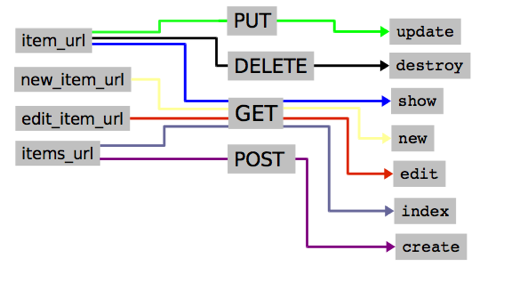
\includegraphics[width=5.0in]{rest}
    \caption{REST[4]}
    \label{REST}
\end{figure}

\item [JWT] : JSON Web Tokens[5], prononcé "JOT", est un standard puisque l'information qu'il transport est transmise via JSON.
JSON Web Tokens travaillent pour différents langages de programmation: JWTs travaillent dans .NET, Python, Node.js, Java, PHP, Ruby, Go, JavaScript et Haskell. Ceux-ci peuvent être utilisés dans de nombreux scénarios différents.
JWTs peuvent être passés facilement: Depuis JWTs sont autonomes, ils sont parfaitement utilisés à l'intérieur d'une en-tête HTTP lors de l'authentification d'une API. Vous pouvez également passer à travers l’URL.

\begin{figure}[H]
    \centering
    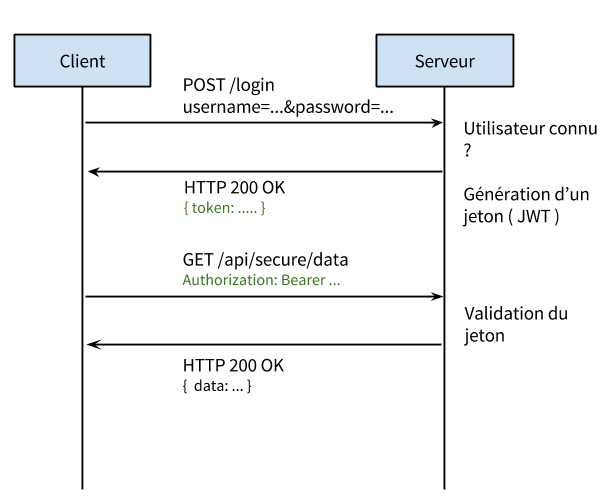
\includegraphics[width=5.0in]{Token-based-Auth}
    \caption{Json Web Token[6]}
    \label{Json Web Token}
\end{figure}
\end{description}

\subsection{Workflow}
La structure du l'application mobile est généré avec YO[10,11], qui crée un projet avec la configuration du GULP.
GULP permet de compiler SASS, Lint JS et de générer une version de production, cette version va être exécutée par les deux runtime (NodeWebkit et Cordova).
Pour mieux contrôler et gérer le code source, GIT est utilisé comme a outil de gestion de versions.
\begin{figure}[H]
    \centering
    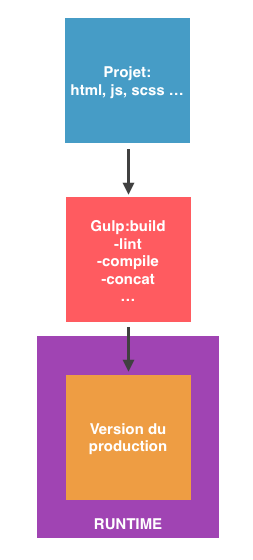
\includegraphics[width=2.5in]{workflow}
    \caption{Structure de projet d'application mobile}
    \label{workflow}
\end{figure}

\section{Implémentation}
\subsubsection{Partie Web}

\begin{figure}[H]
    \centering
    
\includegraphics[width=6in]{screenshots/web/login}
    \caption{Page de connexion}
\end{figure}
Une fois l'administrateur ouvre le site web, la page illustrée dans la figure 5.7 sera affichée, elle permet à l'administrateur de se connecter.
\begin{figure}[H]
    \centering
    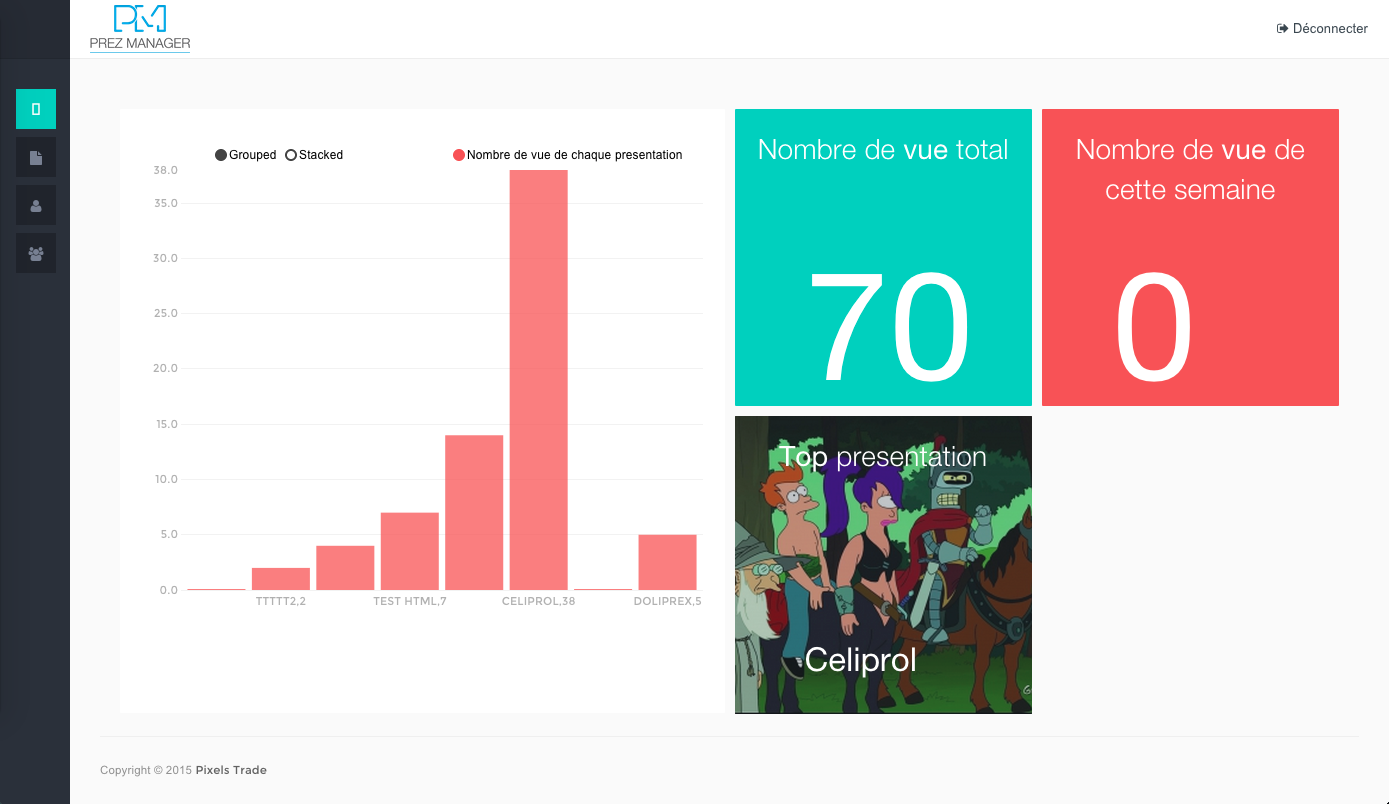
\includegraphics[width=6in]{screenshots/web/home}
    \caption{Page d'accueil}
\end{figure}
La figure 5.8 représente la page d'accueil de site web quand l'administrateur est connecté, elle contient des statistiques générales comme le nombre de vues total, par semaine, le top des présentations.

\begin{figure}[H]
    \centering
    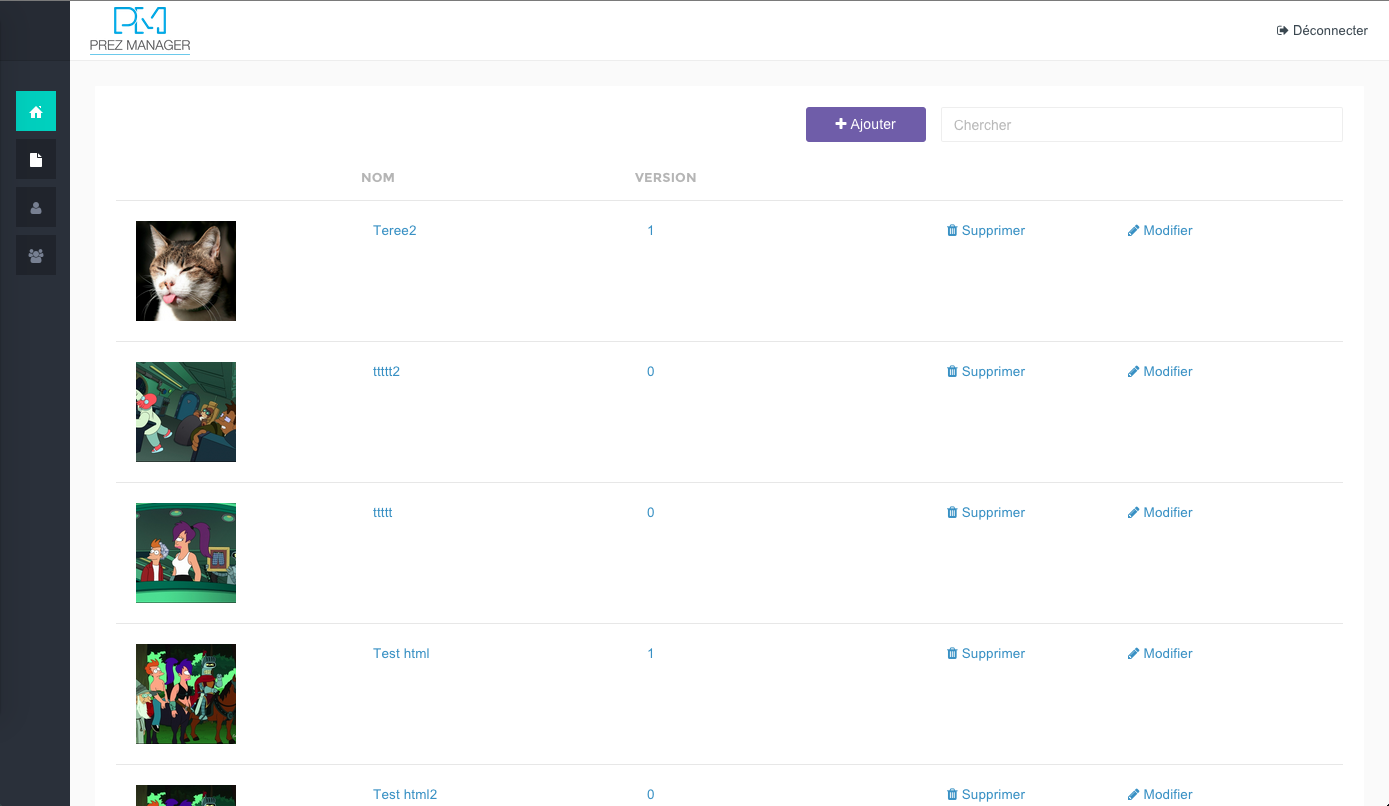
\includegraphics[width=6in]{screenshots/web/listepresentation}
    \caption{Page de liste de présentations}
\end{figure}
La page de liste de présentations est présenté dans la figure 5.9, elle permet d'ajouter, modifier et supprimer les présentations. 

\begin{figure}[H]
    \centering
    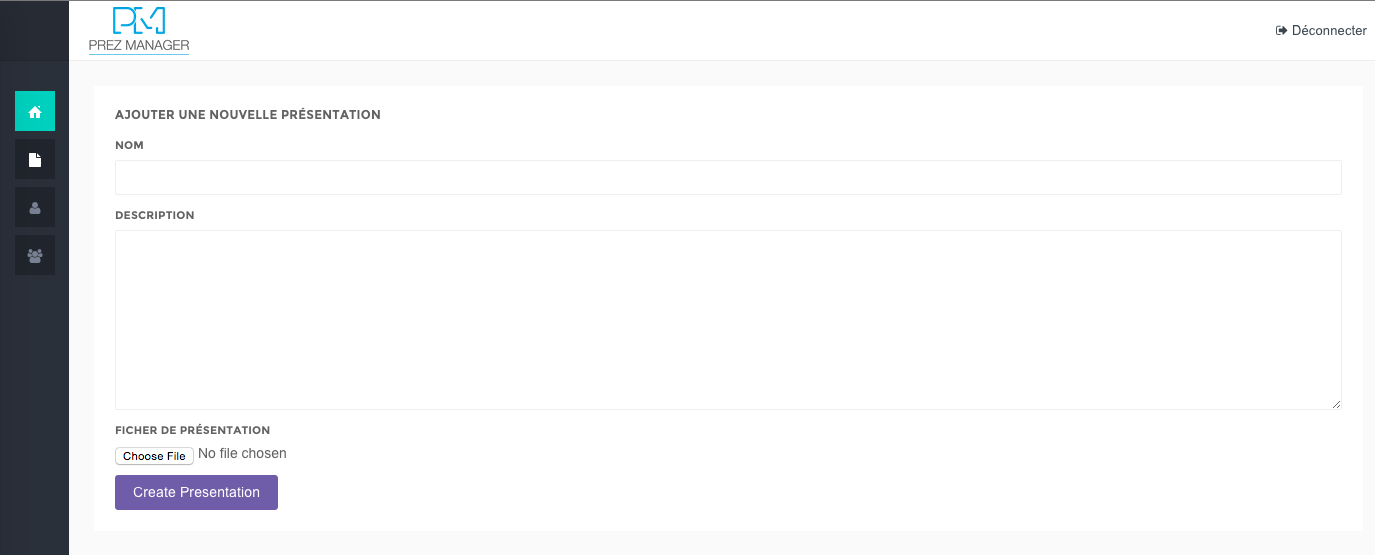
\includegraphics[width=6in]{screenshots/web/ajoutpresentation}
    \caption{Page d'ajoute présentation}

\end{figure}
La figure 5.10 présente la page qui, permet d'ajouter une présentation, En précisant sa nom et description et en sélectionnant la fichier ZIP de présentation.
\begin{figure}[H]
    \centering
    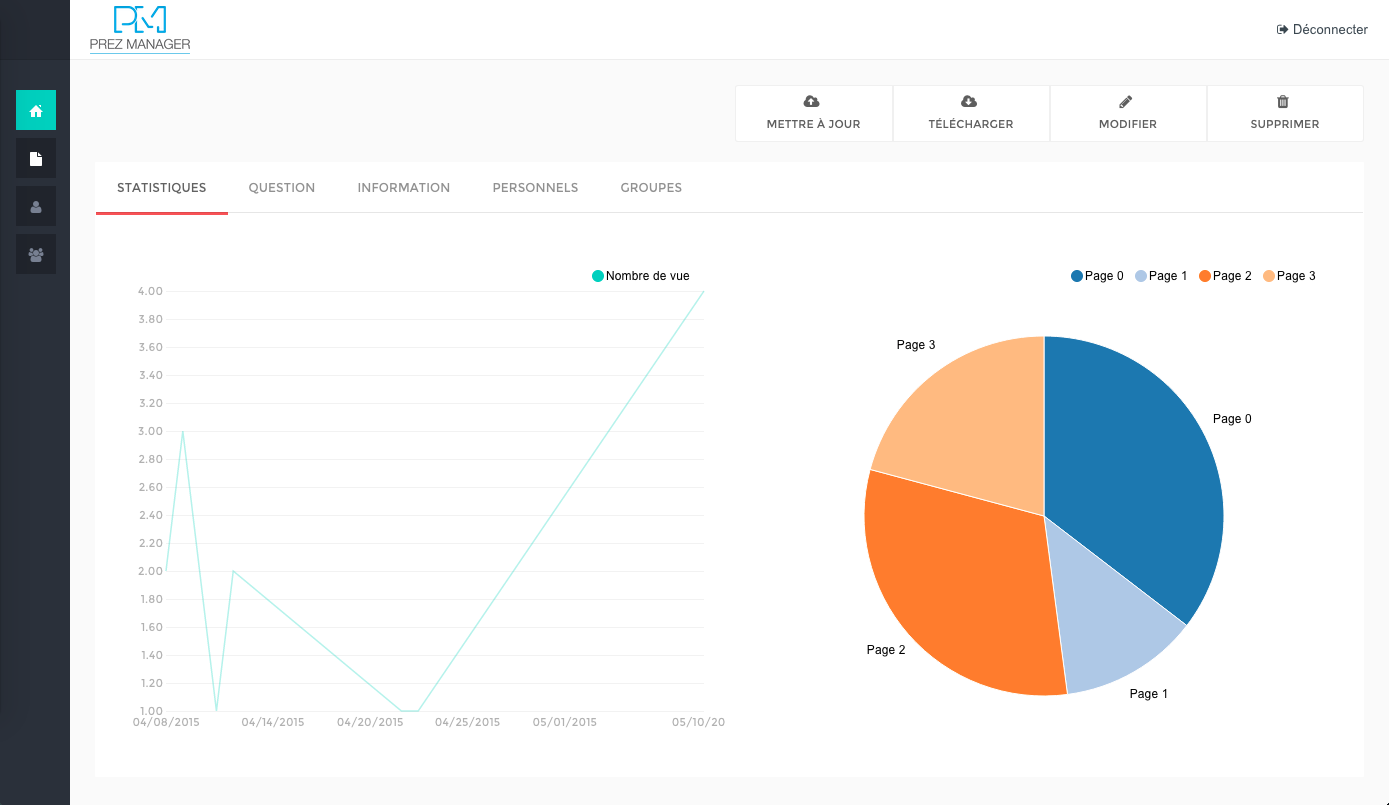
\includegraphics[width=6in]{screenshots/web/statistiquepresentation}
    \caption{Page d'une présentation : onglet statistique}

\end{figure}


Un exemple d'affichage de statistiques de présentation est exposé dans la figure 5.11 La charte et le graphique présentent respectivement le nombre de visualisations par jour et les délais passés dans chaque page de présentation.

\begin{figure}[H]
    \centering
    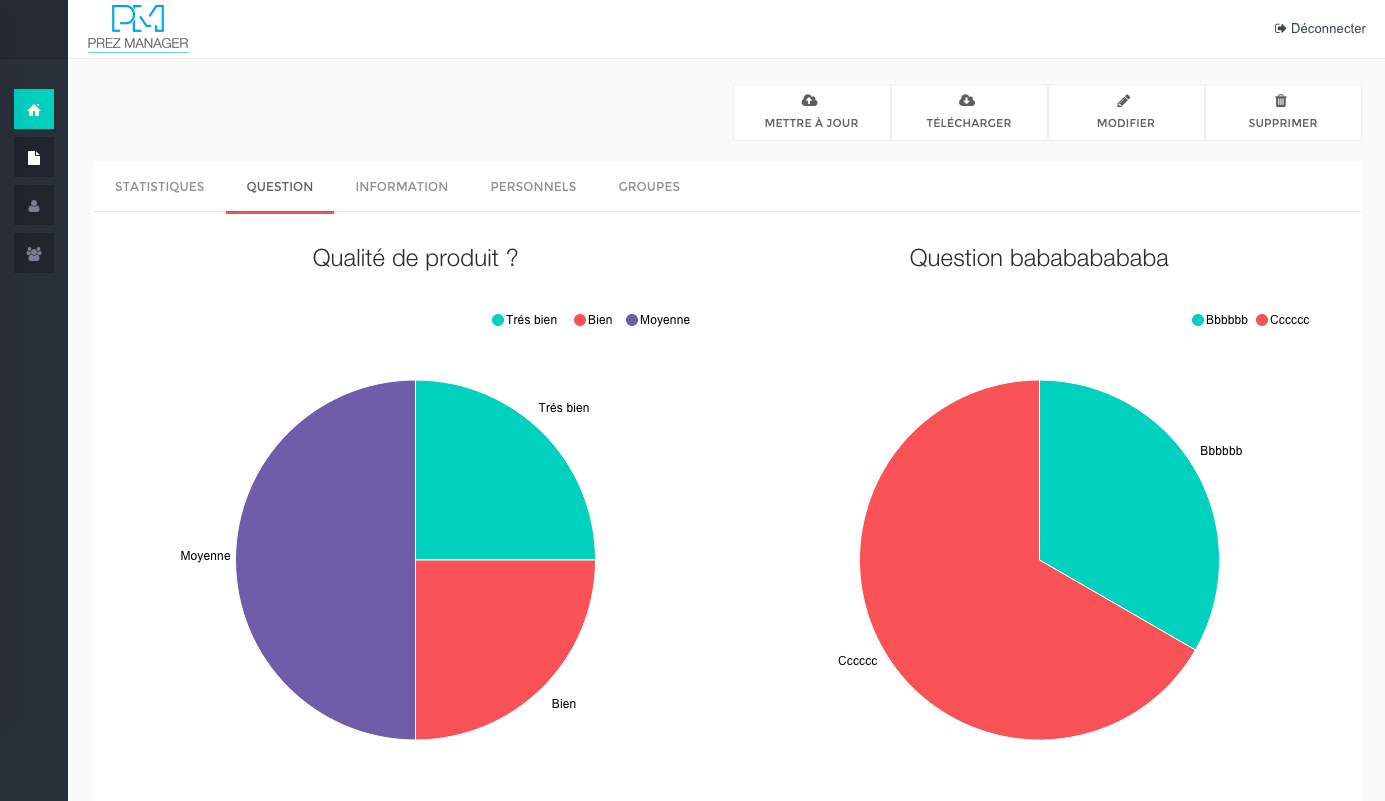
\includegraphics[width=6in]{screenshots/web/prezquestion}
    \caption{Page d'une présentation : onglet question}

\end{figure}

La visualisation des réponses aux questionnaires se fait par des diagrammes circulaires comme le démontre la figure 5.12

\begin{figure}[H]
    \centering
    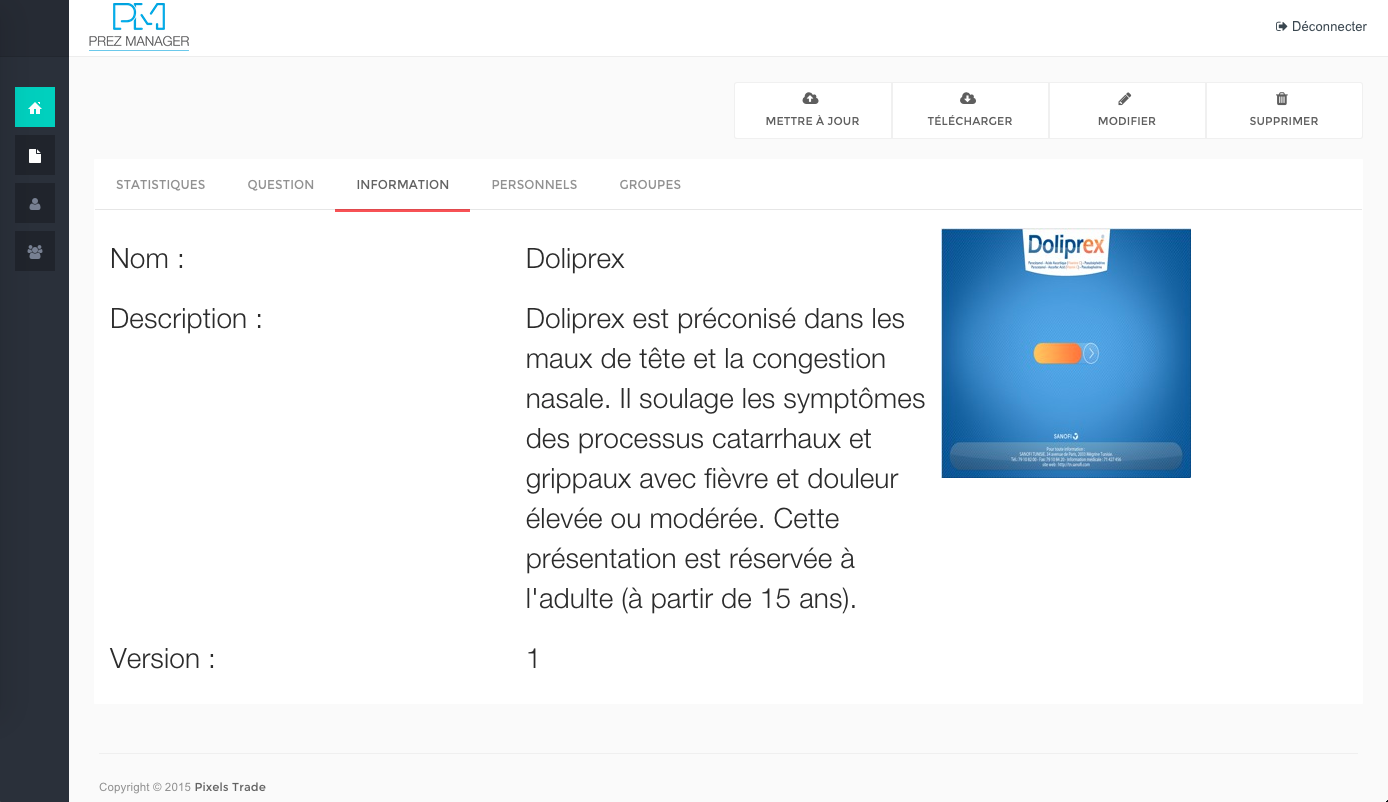
\includegraphics[width=6in]{screenshots/web/prezinfo}
    \caption{Page d'une présentation : onglet information}

\end{figure}

L'onglet information (figure 5.13) contient la description et la version relatives à un produit  particulier.

\begin{figure}[H]
    \centering
    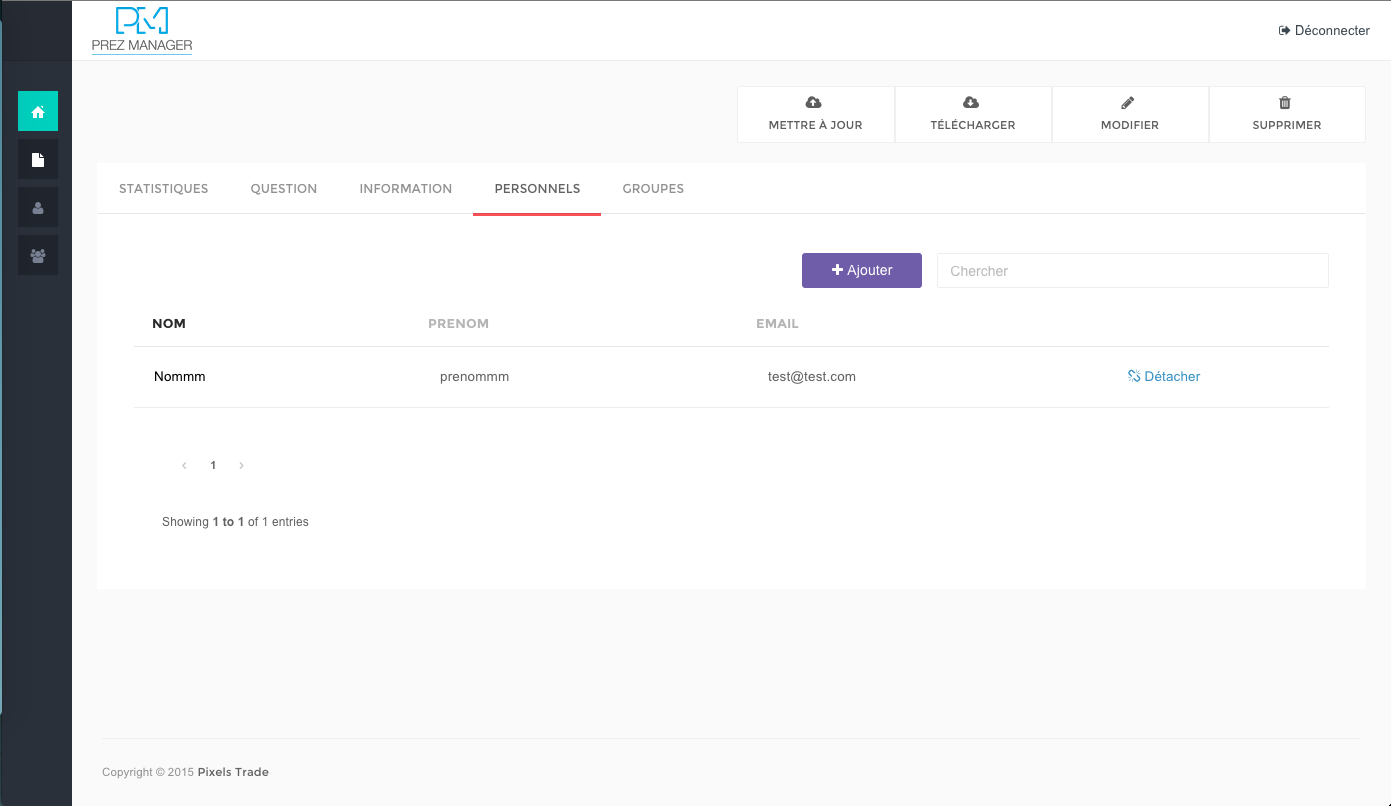
\includegraphics[width=6in]{screenshots/web/prezpersonnel}
    \caption{Page d'une présentation : onglet personnel}

\end{figure}

Chaque présentation est associée à les personnel la présente la figure 5.14.

\begin{figure}[H]
    \centering
    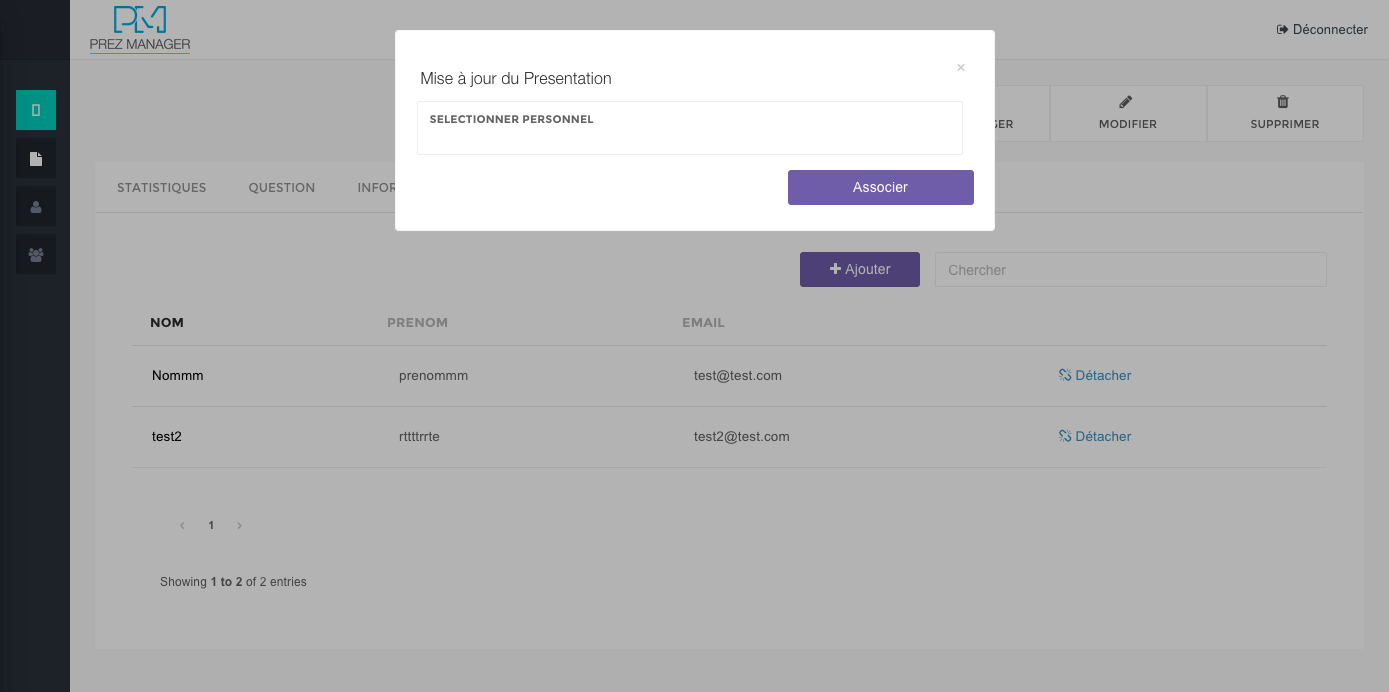
\includegraphics[width=6in]{screenshots/web/popuppersonnel}
    \caption{Page d'une présentation : popup d'ajout du personnel}

\end{figure}

La popup présenté dans la figure 5.15 permet d'associer les présentations aux personnels. 


\begin{figure}[H]
    \centering
    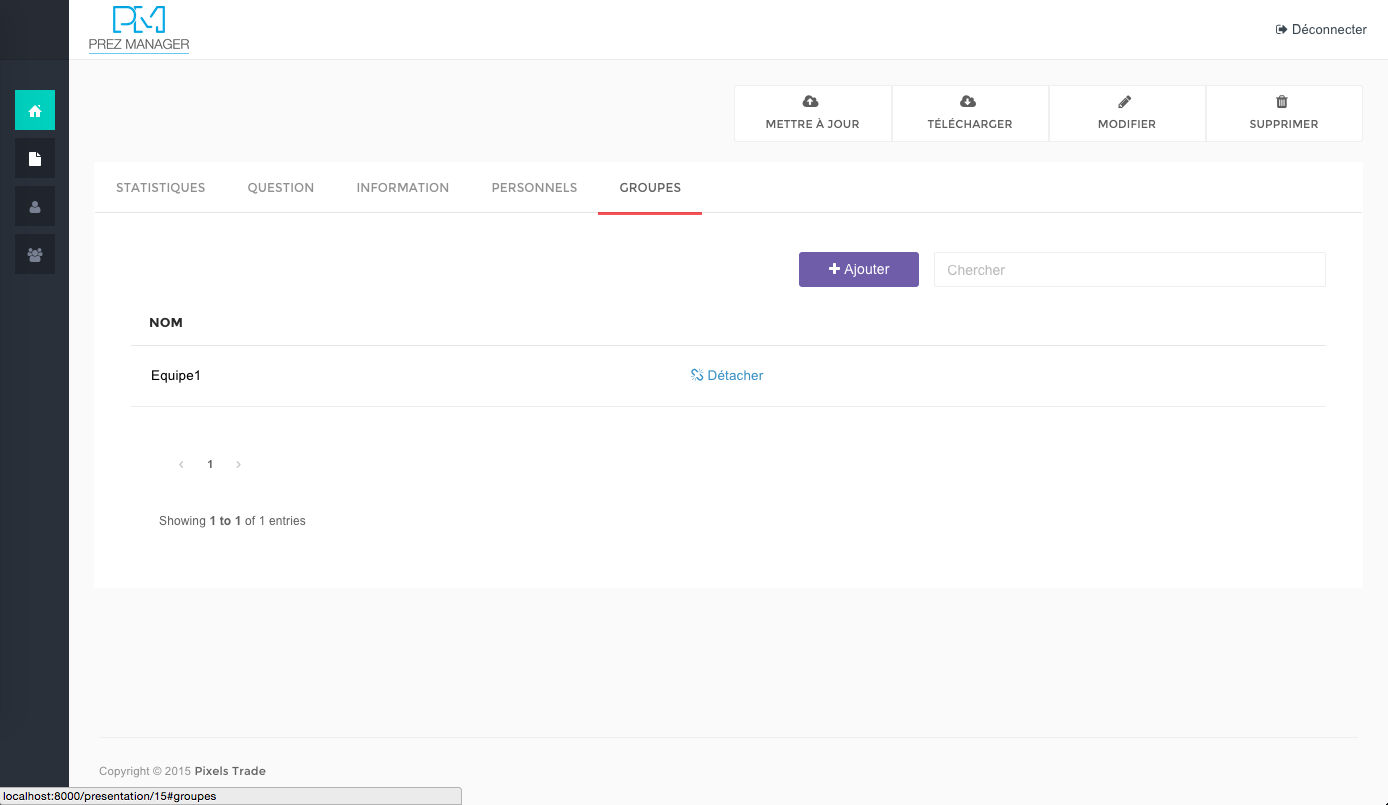
\includegraphics[width=6in]{screenshots/web/prezgroupe}
    \caption{Page d'une présentation : onglet groupes}

\end{figure}

Chaque présentation est associée à des groupes, qui sont listés comme le présente la figure 5.16.

\begin{figure}[H]
    \centering
    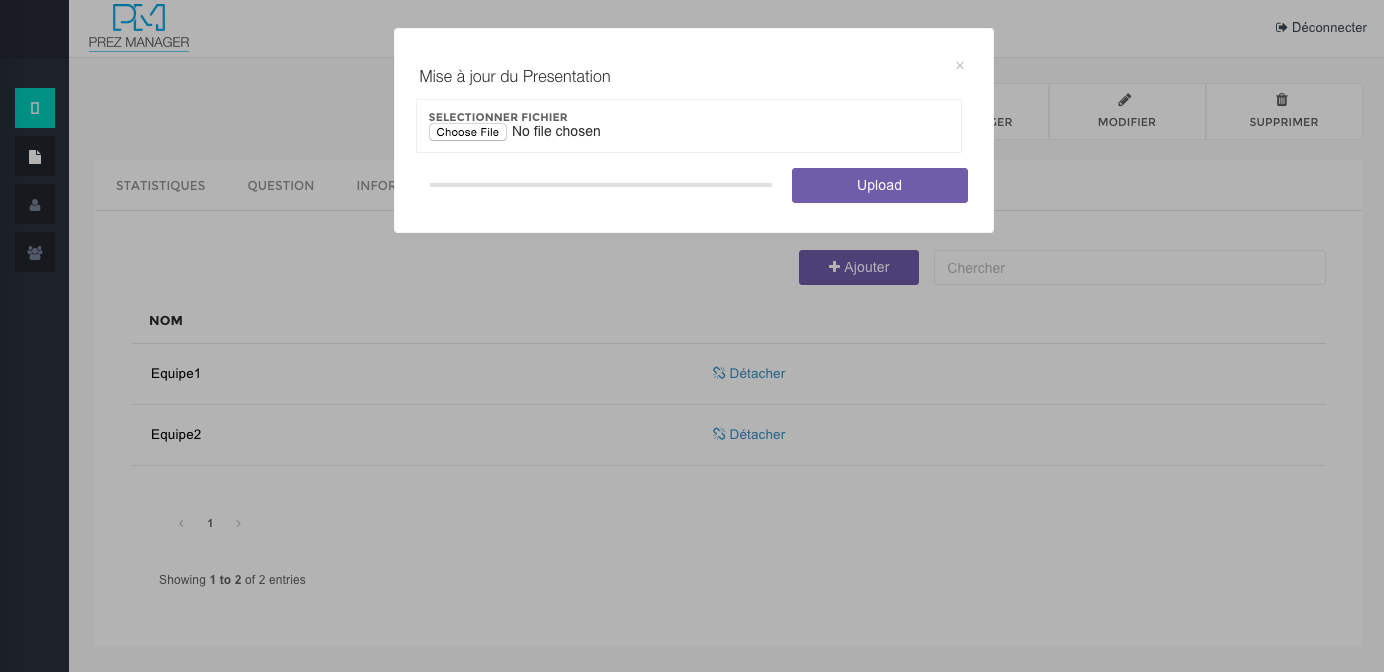
\includegraphics[width=6in]{screenshots/web/updateprez}
    \caption{Page d'une présentation : popup de mise à jour}

\end{figure}

La mise à jour du présentation se fait par le formulaire de la popup affichée dans la figure 5.17.

\begin{figure}[H]
    \centering
    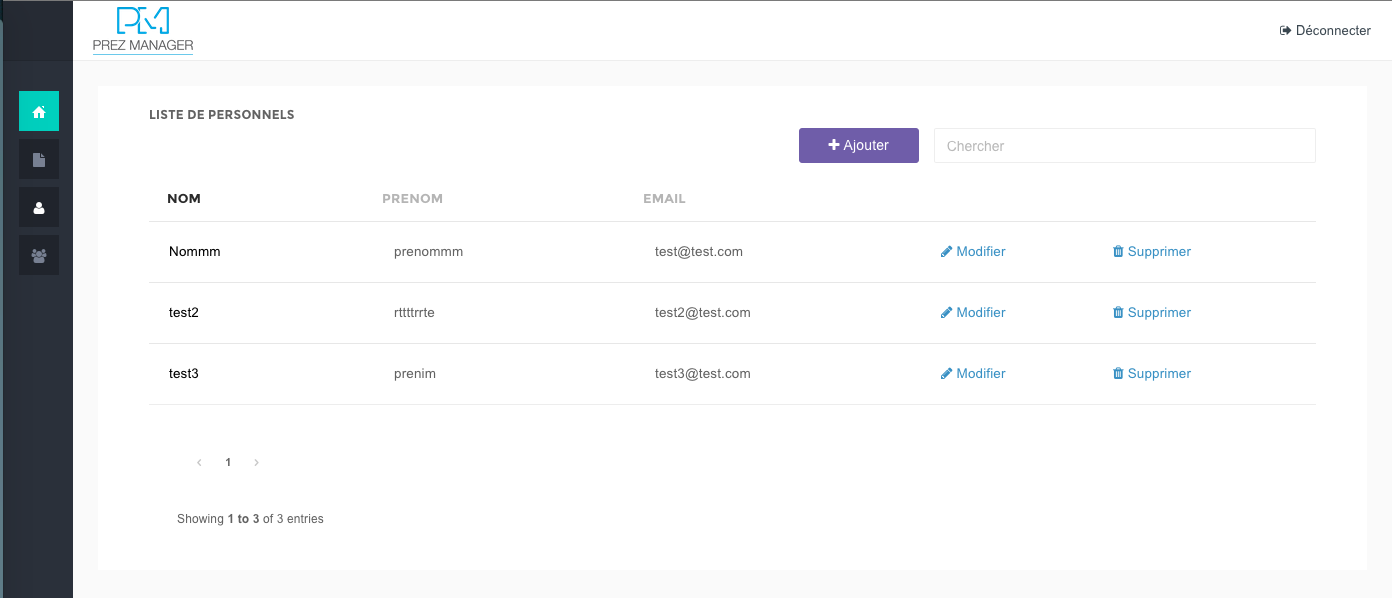
\includegraphics[width=6in]{screenshots/web/listepersonnel}
    \caption{Page liste de personnels}
\end{figure}
La page de liste de personnels est présenté dans la figure 5.18, elle permet de les ajouter, modifier et supprimer. 

\begin{figure}[H]
    \centering
    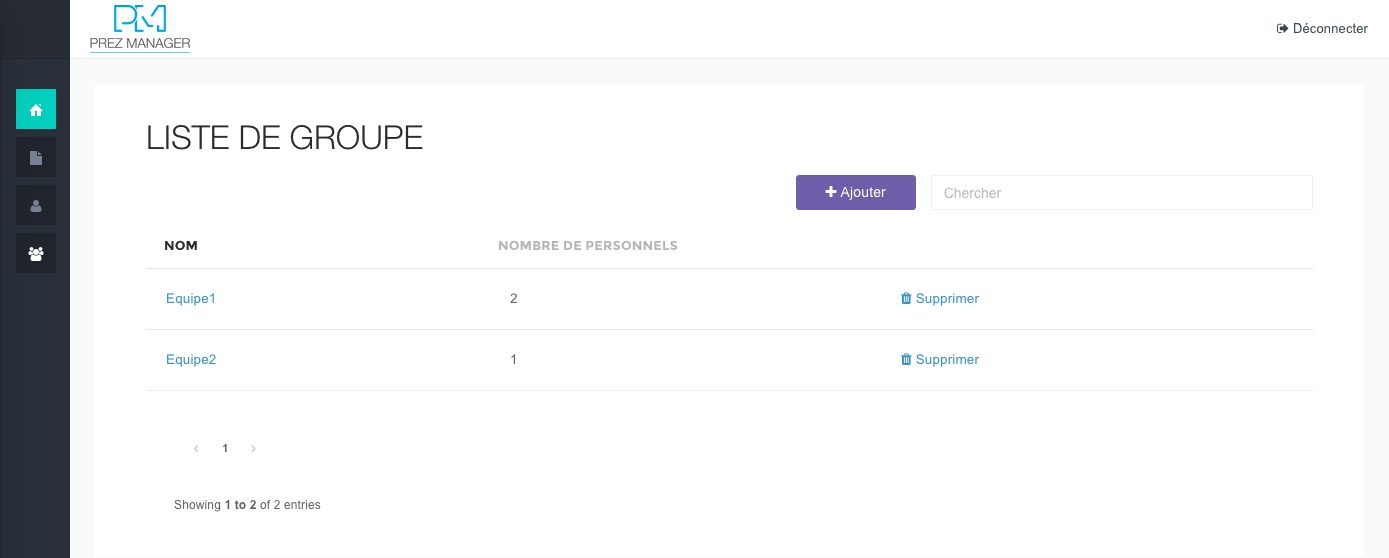
\includegraphics[width=6in]{screenshots/web/listedegroupe}
    \caption{Page liste de groupes}

\end{figure}

La figure 5.19 visualise la page de liste de groupes.

\begin{figure}[H]
    \centering
    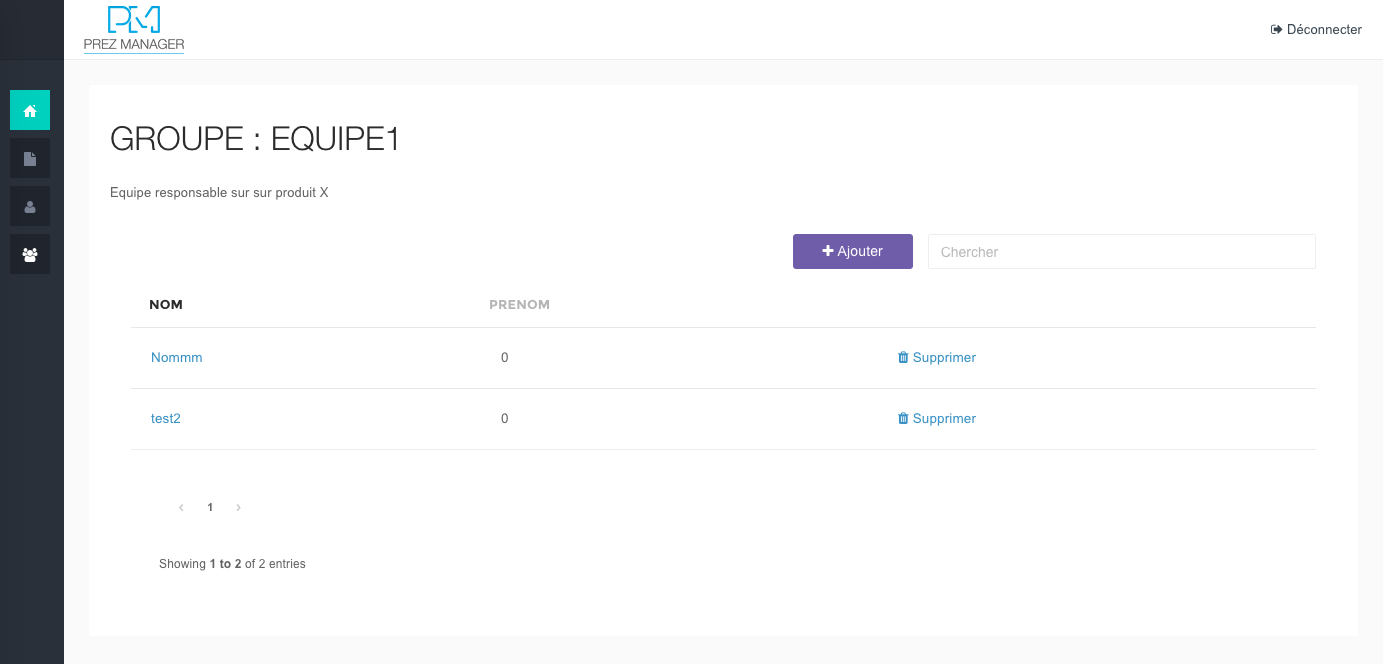
\includegraphics[width=6in]{screenshots/web/pagegroupe}
    \caption{Page de gestion d'un groupe}

\end{figure}
Pour chaque groupe, on peut ajouter ou supprimer du personnel comme l'illustre la figure 5.20.

\subsubsection{Application mobile}

\begin{figure}[H]
    \centering
    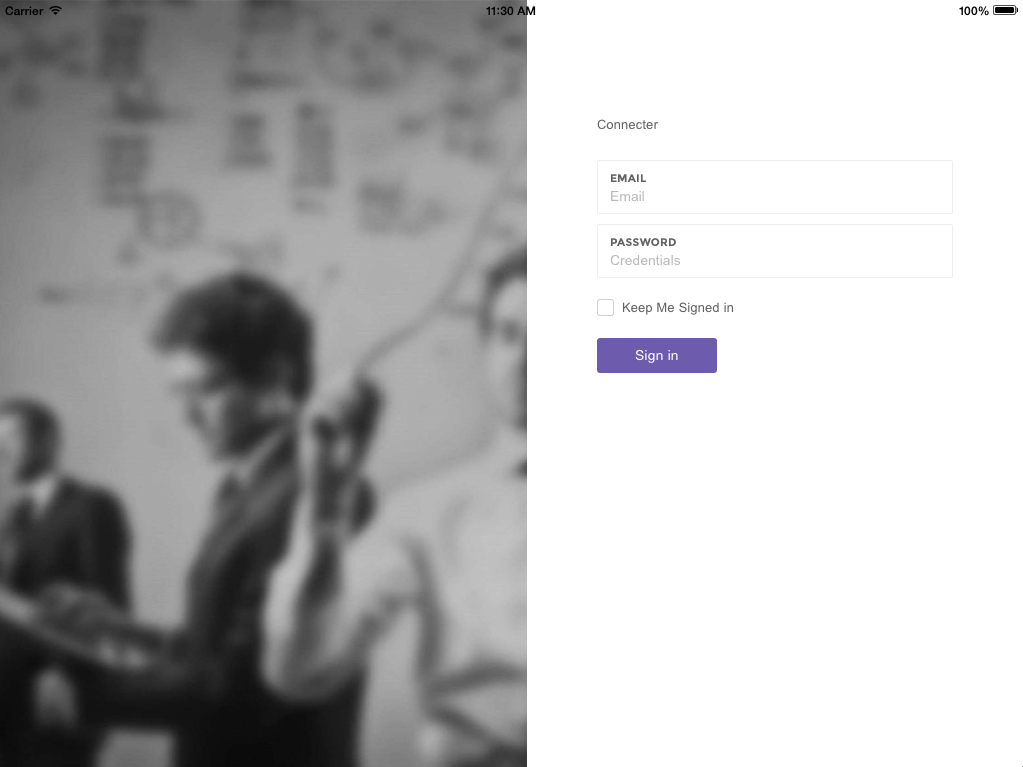
\includegraphics[width=6in]{screenshots/a1}
    \caption{Page de connexion}

\end{figure}

La figure 5.22 présente la première interface graphique qui sera affichée en ouvrant l'application mobile. Elle permet au personnel de se connecter.

\begin{figure}[H]
    \centering
    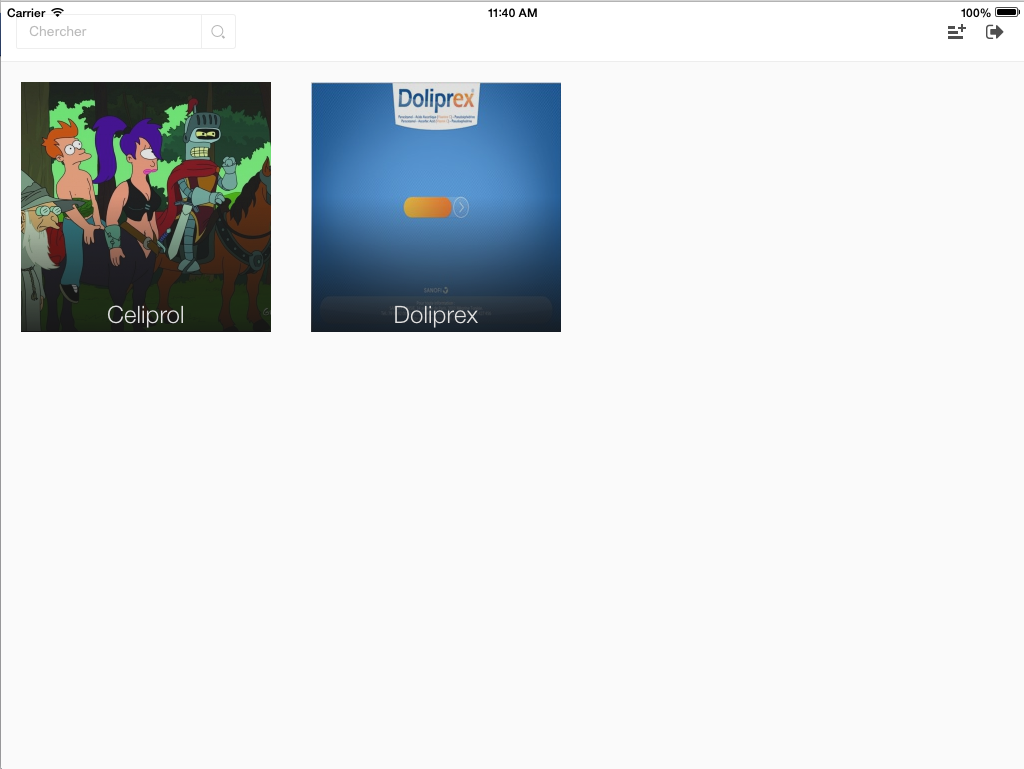
\includegraphics[width=6in]{screenshots/a2}
    \caption{Page liste des présentations en local}
\end{figure}
Les présentations disponibles en local sont visualisées comme l'indique la figure 5.22.

\begin{figure}[H]
    \centering
    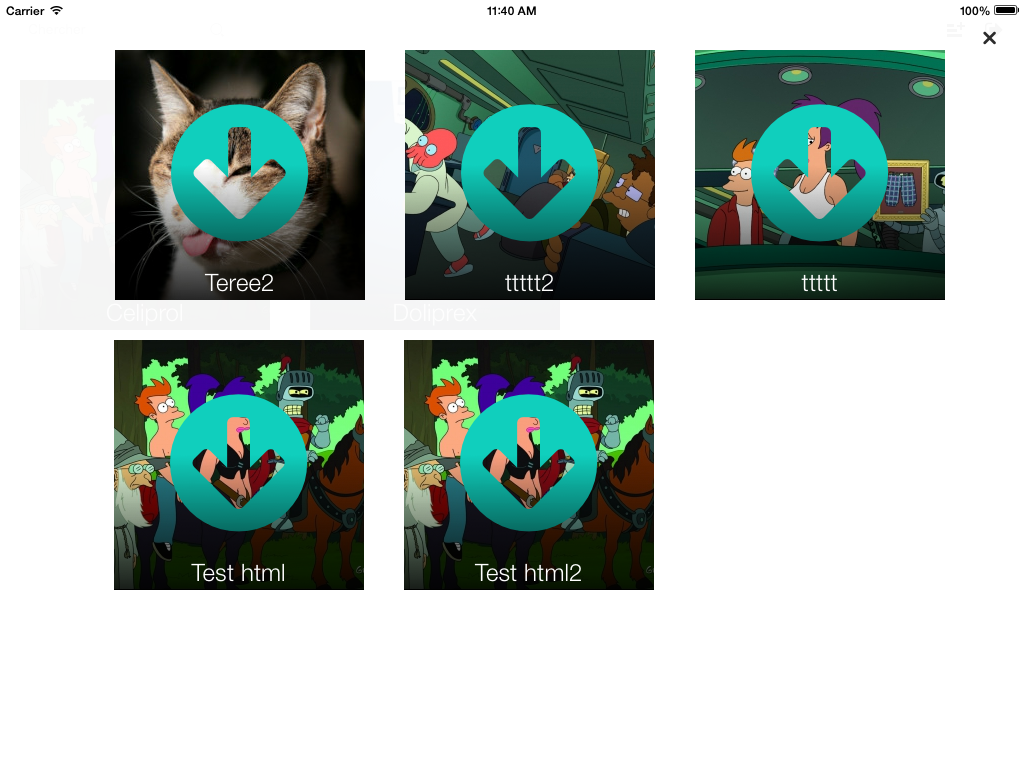
\includegraphics[width=6in]{screenshots/a3}
    \caption{Page liste des présentations disponible à télécharger}
\end{figure}
La liste de présentations qui peuvent être téléchargées est illustrée par la figure 5.23.

\begin{figure}[H]
    \centering
    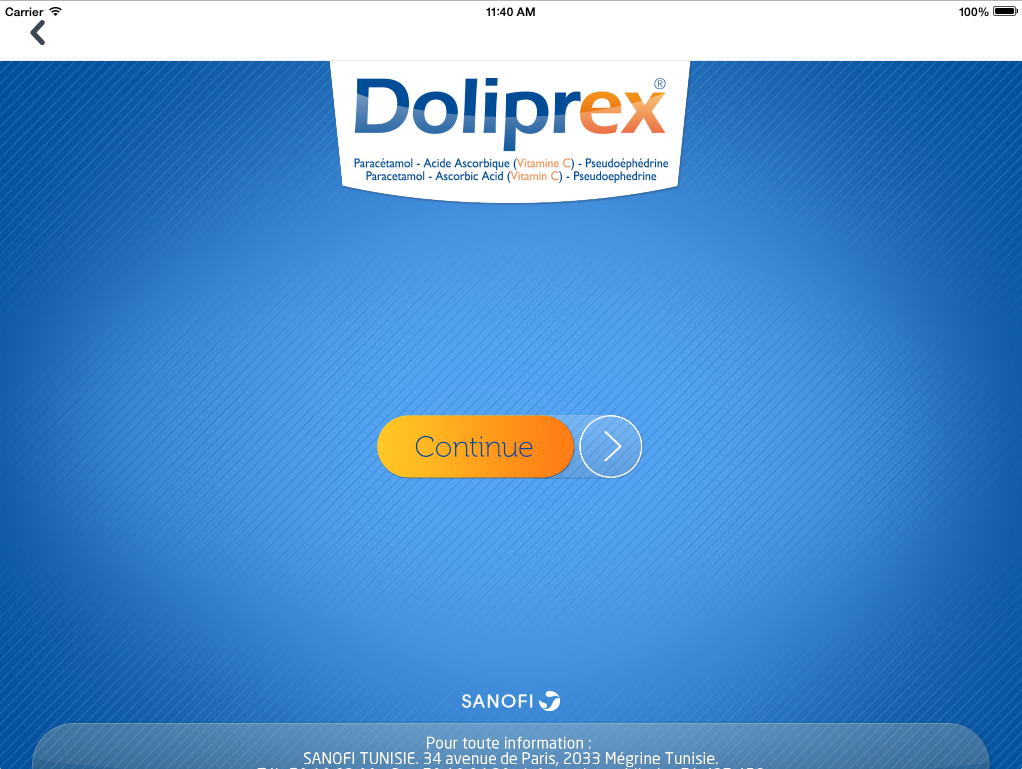
\includegraphics[width=6in]{screenshots/a4}
    \caption{Page de visualisation du présentation}
\end{figure}
La figure 5.24 présente un exemple de visualisation d'une présentation locale.




\section{Conclusion}
À ce stade, nous atteignons la fin de l'étude du projet. Ce dernier chapitre nous a servi à présenter les résultats de la réalisation et de l’intégration de notre solution.


Nous avons commencé par dévoiler l’environnement logiciel, qui nous a permis d’implémenter, de tester et d’intégrer notre plateforme.
Ensuite, nous avons décrit les principales fonctionnalités en illustrant quelque capture écran afin de donner une meilleure idée sur le travail réalisé.


La prochaine étape consiste à clôturer notre rapport par la conclusion générale et les différentes perspectives recensées.
\Conclusion{Conclusion générale} \label{Conclusion}
\PARstart{L}{e} présent rapport a détaillé les étapes effectuées pour mettre en place une plateforme de gestion et visualisation des présentations pour les commerciaux. Afin d’aboutir à ce résultat, nous avons d’abord commencé par la présentation des différents besoins et exigences relevés. Ensuite, nous avons présenté la conception en commençant par l’architecture adoptée, pour aboutir par la suite à une conception détaillée, qui met l’accent sur la partie web et mobile de la plateforme. Enfin nous avons abordé l’étape de réalisation au cours de laquelle nous avons traduit notre modélisation conceptuelle en une implémentation physique moyennant les différentes technologies et technique choisies.

Ce travail nous a été très instructif de point de vue connaissance acquises.
Au niveau fonctionnel, il nous a donné l’occasion d’avoir une idée approfondie sur les méthodes de synchronisation des données entre deux systèmes d’information, la manipulation et sécurisation des web-services. Techniquement, il nous a procuré l’opportunité pour confirmer nos connaissances dans le développement Php et HTML5 et surtout de toucher à plusieurs cycles de vie d’un site web et d’une application mobile tels que la mise en place de l’environnement de travail, la phase de test et le déploiement.
De plus ce travail a été très enrichissant puisqu’il nous a donné l’occasion d’étudier et d’utiliser une panoplie de technologie (Laravel, AngularJS, NodeWebkit, Cordova, etc.) et d’outils (Gulp , composer, GIT, etc.)


Hormis le côté technique et fonctionnel, ce projet a été une opportunité pour appréhender le travail dans une hiérarchie professionnelle au sein d’une grande société et les difficultés inhérentes comme la répartition du temps et des efforts. En participant au développement du projet, nous avons pu découvrir la rigueur nécessaire à la satisfaction du client ainsi que les bonnes pratiques nécessaires à la réalisation d’un produit de qualité.



Pour conclure, la solution développée constitue une première version de la plateforme de gestion des présentations, dans laquelle nous avons tracé les grandes lignes des fonctionnalités proposées par la société d'accueil.


Nous souhaitons, enfin que ce modeste travail apporte progrès, évolution et satisfaction aux responsables de Pixels Trade, aux membres du jury et à toute personne intéressée par le domaine de digitalisation, de la gestion des présentations et de l’amélioration des ventes.
\Remerciements{Bibliographie}
\large
\vspace{6mm}
\begin{enumerate}
\item Claude Aubry. Scrum : Le guide pratique de la methode agile la plus populaire. Dunod, 2009.
\item Ari Lerner. Ng-book : The Complete Book on AngularJS.
\item Kyle Simpson. You Don't Know JS: Scope \& Closures.
\end{enumerate}


\Remerciements{Netographie}

\large
\vspace{6mm}
\begin{enumerate}
    \setcounter{enumi}{3}
    \item dablog.rubypal.com/2008/11/24/restful-rails-for-the-restless
    
    \item www.jwt.io
    \item maxlab.fr/2014/05/gerer-lauthentification-dune-application-javascript/

    \item cordova.apache.org/docs/en/5.0.0/
    \item www.nwjs.io

    
    \item laravel.com/docs/5.0

    \item www.yeoman.io
    \item github.com/Swiip/generator-gulp-angular
    \item www.google.com/trends
    \item www.sitepoint.com/best-php-framework-2015-sitepoint-survey-results
    \item docs.angularjs.org/guide
    \item github.com/djyde/StoreDB
    

\end{enumerate}


\end{document}
